% --- Template for thesis / report with tktltiki2 class ---
%
% last updated 2013/02/15 for tkltiki2 v1.02

\documentclass[12pt,finnish]{tktltiki2}

% tktltiki2 automatically loads babel, so you can simply
% give the language parameter (e.g. finnish, swedish, english, british) as
% a parameter for the class: \documentclass[finnish]{tktltiki2}.
% The information on title and abstract is generated automatically depending on
% the language, see below if you need to change any of these manually.
%
% Class options:
% - grading                 -- Print labels for grading information on the front page.
% - disablelastpagecounter  -- Disables the automatic generation of page number information
%                              in the abstract. See also \numberofpagesinformation{} command below.
%
% The class also respects the following options of article class:
%   10pt, 11pt, 12pt, final, draft, oneside, twoside,
%   openright, openany, onecolumn, twocolumn, leqno, fleqn
%
% The default font size is 11pt. The paper size used is A4, other sizes are not supported.
%
% rubber: module pdftex

% --- General packages ---

\usepackage[utf8]{inputenc}
\usepackage[T1]{fontenc}
\usepackage{lmodern}
\usepackage{microtype}
\usepackage{amsfonts,amsmath,amssymb,amsthm,booktabs,color,enumitem,graphicx}
\usepackage[pdftex,hidelinks]{hyperref}

\usepackage{url}
\usepackage{setspace}
\onehalfspacing

\setlength{\parskip}{1ex} % kappaleiden välinen tyhjä tila
\setlength{\parindent}{0pt} % kappaleen alun sisennys

% Automatically set the PDF metadata fields
\makeatletter
\AtBeginDocument{\hypersetup{pdftitle = {\@title}, pdfauthor = {\@author}}}
\makeatother

% --- Language-related settings ---
%
% these should be modified according to your language

% babelbib for non-english bibliography using bibtex
\usepackage[fixlanguage]{babelbib}
\selectbiblanguage{finnish}

% add bibliography to the table of contents
\usepackage[nottoc]{tocbibind}
% tocbibind renames the bibliography, use the following to change it back
\settocbibname{Lähteet}

% --- Theorem environment definitions ---

\newtheorem{lau}{Lause}
\newtheorem{lem}[lau]{Lemma}
\newtheorem{kor}[lau]{Korollaari}

\theoremstyle{definition}
\newtheorem{maar}[lau]{Määritelmä}
\newtheorem{ong}{Ongelma}
\newtheorem{alg}[lau]{Algoritmi}
\newtheorem{esim}[lau]{Esimerkki}

\theoremstyle{remark}
\newtheorem*{huom}{Huomautus}

\makeatletter
\g@addto@macro\@floatboxreset\centering
\makeatother


% --- tktltiki2 options ---
%
% The following commands define the information used to generate title and
% abstract pages. The following entries should be always specified:

\title{Normalisoitu pakkausetäisyys: sovelluksia ja variaatioita}
\author{Timo Sand}
\date{\today}
\level{Kandidaatintutkielma}
\abstract{
Tähän tulee tutkielman tiivistelmä
\begin{itemize}
  \item NCD:n esittely
  \item Klusteroinnin esittely
  \item Ongelma ja Ominaisuudet
  \item GSD
\end{itemize}
} % TODO: Tiivistelmä

% The following can be used to specify keywords and classification of the paper:

\keywords{Samankaltaisuus, Klusterointi, Valvomaton oppiminen, Tiedonlouhinta}

% classification according to ACM Computing Classification System (http://www.acm.org/about/class/)
% This is probably mostly relevant for computer scientists
% uncomment the following; contents of \classification will be printed under the abstract with a title
% "ACM Computing Classification System (CCS):"
\classification{\textbf{Information systems - Similarity measures} \\ \textit{Theory of computation - Unsupervised learning and clustering} \\ Data mining - Clustering}

% If the automatic page number counting is not working as desired in your case,
% uncomment the following to manually set the number of pages displayed in the abstract page:
%
% \numberofpagesinformation{16 sivua + 10 sivua liitteissä}
%
% If you are not a computer scientist, you will want to uncomment the following by hand and specify
% your department, faculty and subject by hand:
%
% \faculty{Matemaattis-luonnontieteellinen}
% \department{Tietojenkäsittelytieteen laitos}
% \subject{Tietojenkäsittelytiede}
%
% If you are not from the University of Helsinki, then you will most likely want to set these also:
%
% \university{Helsingin Yliopisto}
% \universitylong{HELSINGIN YLIOPISTO --- HELSINGFORS UNIVERSITET --- UNIVERSITY OF HELSINKI} % displayed on the top of the abstract page
% \city{Helsinki}
%

\newcommand{\engl}[1]{\emph{(engl. #1)}}
\newcommand{\kolmogorov}{Kolmogorov-kompleksisuus}


\begin{document}

% --- Front matter ---

\frontmatter      % roman page numbering for front matter

\maketitle        % title page
\makeabstract     % abstract page

\tableofcontents  % table of contents

% --- Main matter ---

\mainmatter       % clear page, start arabic page numbering

\section{Johdanto} % (fold)
\label{sec:johdanto}
\label{par:intro-1}
  Kaikki data on luotu samanveroiseksi, mutta jotkut datat ovat samankaltaisempia kuin toiset.
  Esitämme tavan, jolla ilmaista tämä samankaltaisuus, käyttäen Cilibrasin ja Vitanyin esittelemää samankaltaisuuden metriikkaa \engl{similarity metric}, joka perustuu tiedoston pakkaamiseen. \cite{CV05}
  Metriikka on parametriton, eli se ei käytä datan ominaisuuksia tai taustatietoja, ja sitä voi soveltaa eri aloihin ilman muunnoksia.
  Metriikka on universaali siten, että se approksimoi parametrin, joka ilmaisee parin hallitsevan piirteen samankaltaisuutta pareittain vertailuissa.
  Se on vakaa siinä mielessä, että sen tulokset ovat riippumattomia käytetystä pakkaajasta \cite{CV05}. Pakkaajalla tarkoitetaan pakkausohjelmaa kuten \emph{gzip, ppmz, bzip2}.

  \label{par:intro-2}
  Pakkaukseen perustuva samankaltaisuus \engl{Compression-Based Similarity} on universaali metriikka, jonka kehittivät Cilibrasi ja Vitanyi \cite{CV05}.
  Yksinkertaistettuna tämä tarkoitta, että kaksi objektia ovat lähellä toisiaan, jos voimme ``pakata'' yhden objektin huomattavasti tiiviimmin toisen objektin datalla.
  Abstraktina ideana toimii se, että voimme kuvailla ytimekkäämmin yhden objektin toisen avulla, mikäli objektit ovat samankaltaisia.
  Tämän esittelemme luvussa \ref{sec:normalisoitu_pakkausetaisyys} ja samalla käymme läpi, mihin teoriaan algoritmi perustuu sekä miten se toimii.
  Edellä mainitun vakauden esittämiseen voimme käyttää useaa tosielämän pakkausalgoritmia: tilastollista (PPMZ), Lempel-Ziv -algoritmiin pohjautuvaa hakemistollista (gzip), lohkoperusteista (bzip2) tai erityistarkoitusta varten suunniteltua (Gencompress).

  Kaikissa kohdissa  operoimme $O(log n)$ tarkkuudella, joka on hinta siitä että siirrytään Kolmogorov-kompleksisuudesta laskettavaan approksimaatioon.

  Tarkoituksemme on koota yhteen samankaltaisuuden metriikkaan kaikki tehokkaat etäisyydet \engl{effective distances}: tehokkaat versiot Hammingin etäisyydestä, Euklidisesta etäisyydestä, Lempel-Ziv etäisyydestä ja niin edelleen.
  Tämän metriikan tulee olla niin yleinen, että se toimii yhtäläisesti ja samanaikaisesti kaikilla aloilla: musiikilla, tekstillä, kirjallisuudella, ohjelmilla, genomeilla, luonnollisen kielen määrityksillä.
  Sen pitäisi pystyä samanaikaisesti havaitsemaan kaikki samankaltaisuudet objektien välillä, joita muut etäisyydet havaitsevat erikseen.

  Kun määrittelemme ryhmän sallittavia etäisyyksiä \engl{admissible distances} haluamme sulkea pois epärealistiset, kuten $f(x,y) = \frac{1}{2}$ jokaiselle parille $x \neq y$.
  Saavutamme tämän rajoittamalla objektien lukumäärän annetussa etäisyydessä objektiin.
  Teemme tämän huomioimalla vain todellisia etäisyyksiä seuraavasti: Oletamme kiinnitetyn ohjelmointikielen, joka toimii tutkielman ajan viitekielenä.
  Tämä ohjelmointikieli voi olla yleinen kieli kuten LISP, Ruby tai se voi myös olla kiinnitetty universaali Turingin kone. \cite{CV05,cilibrasi2007google}
  Valinnalla ei kuitenkaan ole merkitystä, sillä teoria on invariantti ohjelmointikielin muutoksille, kunhan pysytään tehdyssä valinnassa.


Jotta voimme soveltaa tätä ideaalia ja tarkkaa matemaattista teoriaa käytäntöön, pitää meidän korvata ei laskettavissa oleva Kolmogorov-kompleksisuus approksimaatiolla käyttäen standardia pakkaajaa.

\label{par:intro-3}
  Luvussa \ref{sec:klusterointi} esittelemme algoritmin käyttöä klusteroinnissa.
  Aloitamme siitä, miten yleisesti \emph{Normalisoidun pakkausetäisyyden} (\emph{NCD}) avulla pystymme klusteroimaan tuloksia eri kategorioihin; miten musiikkikappaleet klusteroituvat saman artistin alle, miten kuvantunnistuksessa saamme ryhmitettyä samankaltaiset kuvat ja miten sienten genomeista saamme tarkan lajiryhmityksen.


  Luvun lopussa syvennymme musiikin, kuvantunnistuksen ja dokumenttien kategorisoinnin tuloksiin.


\label{par:intro-4}
  Luvussa \ref{sec:algoritmin_ongelmat_ja_ominaisuudet} esitellään NCD:n ominaisuuksia ja ongelmia.
  Ensiksi esitellään NCD:n kohinansietokykyä, eli katsotaan mitä tapahtuu kun lisätään vähitellen kohinaa toiseen tiedostoista, jota pakataan, ja mittaamalla samankaltaisuutta tämän jälkeen \cite{4167725}.
  Saamme nähdä miten paljon kohina vaikuttaa NCD:n laskemiin etäisyyksiin ja huonontaako se klusteroinnin tuloksia.


  Mikään algoritmi ei ole täydellinen, ja NCD-algoritmillakin on ongelmansa.
  Algoritmissa itsessään ei ole selvää heikkoutta, mutta sen käytössä on otettava pakkaajan valinta huomioon, koska monet suosituista pakkausalgoritmeista ovat optimoituja tietyn kokoisille tiedostoille.
  Niissä on niin kutsuttu ikkunakoko \engl{window size}, joka määrittelee mikä tiedostokoko on sopiva \cite{cebrian2005common}.
  Jos tiedostokoko on pienempi kuin ikkunakoko, niin pakkaus on tehokasta, mutta kun mennään siitä yli, pakkauksesta tulee huomattavasti tehottomampaa.
  Esittelemme tuloksia eri pakkausalgoritmien vertailuista ja mikä näistä algoritmeista on parhaimmaksi havaittu NCD:n kanssa käytettäväksi.


\label{par:intro-5}
  NCD ei ole ainut metriikka, jolla voidaan mitata samankaltaisuutta.
  Internetiä hyödyntäen on tehty metriikka, joka käyttää hakukoneita samankaltaisuuden tutkimiseen; tämä on nimetty Google-samankaltaisuusetäisyydeksi \engl{Google Similarity Distance}.
  Tämä toimii myös muilla hakukoneilla kuten Bing. Luvussa \ref{sec:google_samankaltaisuusetaisyys} esittelemme tämän.

% section johdanto (end)

\section{Normalisoitu pakkausetäisyys} % (fold)
\label{sec:normalisoitu_pakkausetaisyys}
  \subsection{\kolmogorov} % (fold)
\label{sub:kolmogorov_kompleksisuus}

  Merkkijonon $x$ \emph{\kolmogorov} on pituus bitteinä, lyhimmästä tietokoneohjelmasta joka ilman syötettä palauttaa merkkijonon $x$; tämä merkitään $K(x)=K(x|\lambda)$, $\lambda$ esittää tyhjää syötettä.
  Lyhimmän tietokoneohjelman pituus, joka palauttaa $x$ syötteellä $y$, on \kolmogorov{} $x$:stä syötteellä $y$; tämä merkitään $K(x|y)$.
  Yksi tapa hahmottaa Kolmogorov-kompleksisuutta $K(x)$ on ajatella se pituutena bitteinä $x$:n tiiviimmin pakatussa muodossa, josta voidaan purkaa $x$ pakkauksenpurkuohjelmalla.

% subsection kolmogorov_kompleksisuus (end)
\subsection{Normalisoitu informaatioetäisyys} % (fold)
\label{sub:normalisoitu_informaatioetaisyys}

  Artikkelissa \cite{CV05} on esitelty \emph{informaatioetäisyys} $E(x,y)$, joka on määritelty lyhimpänä binääriohjelman pituutena, joka syötteellä $x$ laskee $y$:n ja syötteellä $y$ laskee $x$:n. Tämä lasketaan seuraavasti:

  \begin{align}
    E(x,y) &= max\{K(x|y),K(y|x)\}.
  \end{align}

  Normalisoitu versio informaatioetäisyydestä $E(x,y)$, jota kutsutaan \emph{normalisoiduksi informaatioetäisyydeksi}, on määritelty seuraavasti

  \begin{align}
    NID(x,y) &= \frac{ max\{K{(x|y)},K{(y|x)}\} }{ max \{K(x),K(y)\}}.
  \end{align}

  Tämä on paras mahdollinen \emph{samankaltaisuuden metriikka}, ja sen on osoitettu \cite{CV05} täyttävän vaatimukset etäisyyden metriikaksi.
  \emph{NID} ei kuitenkaan ole laskettava tai edes semi-laskettava, koska Turingin määritelmän mukaan \kolmogorov{} ei ole laskettava \cite{CV05}.
  Nimittäjän approksimointi annetulla pakkaajalla $C$ on $max \{C(x),C(y)\}$.
  Osoittajan paras approksimaatio on $max\{C(xy),C(yx)\} - \min\{C(x),C(y)\}$ \cite{CV05}.
  Kun \emph{NID} approksimoidaan oikealla pakkaajalla, saadaan tulos jota kutsutaan \emph{normalisoiduksi pakkausetäisyydeksi}.
  Tämä esitellään formaalisti myöhemmin.
% subsection normalisoitu_informaatioetaisyys (end)

\subsection{Normaali pakkaaja} % (fold)
\label{sub:normaali_pakkaaja}

  Seuraavaksi esitämme aksioomia, jotka määrittelevät laajan joukon pakkaajia ja samalla varmistavat \emph{normalisoidussa pakkausetäisyydessä} halutut ominaisuudet.
  Näihin pakkaajiin kuuluvat monet tosielämän pakkaajat.

  Pakkaaja $C$ on \emph{normaali} jos se täyttää seuraavat aksioomat:

  \label{idempotency}
  \begin{enumerate}
    \item \emph{Idempotenssi}: $C(xx) = C(x)$ ja $C(\lambda) = 0$, jossa $\lambda$ on tyhjä merkkijono,
    \item \emph{Monotonisuus}: $C(xy) \geq C(x)$,
    \item \emph{Symmetrisyys}: $C(xy) = C(yx)$ ja
    \item \emph{Distributiivisuus}: $C(xy) + C(z) \leq C(xz) + C(yz)$.
  \end{enumerate}
% subsection normaali_pakkaaja (end)

\subsection{Normalisoitu Pakkausetäisyys} % (fold)
\label{sub:normalisoitu_pakkausetaisyys}

  Jotta voimme soveltaa tätä ideaalia ja tarkkaa matemaattista teoriaa käytäntöön, pitää meidän korvata ei laskettavissa oleva Kolmogorov-kompleksisuus approksimaatiolla käyttäen standardia pakkaajaa.

  Normalisoitua versiota \emph{hyväksyttävästä etäisyydestä} $E_c(x,y)$, joka on pakkaajaan $C$ pohjautuva approksimaatio normalisoidusta informaatioetäisyydestä, kutsutaan nimellä \emph{Normalisoitu Pakkausetäisyys (NCD)} \cite{CV05}.
  Tämä lasketaan seuraavasti

  \begin{align}
    NCD(x,y) &= \frac{C(xy)-min\{C(x),C(y)\}}{max\{C(x),C(y)\}}.
  \end{align}

  \emph{NCD} on funktioiden joukko, joka ottaa argumenteiksi kaksi objektia (esim. tiedostoja tai Googlen hakusanoja) ja tiivistää nämä, erillisinä ja yhdistettyinä.
  Tämä funktioiden joukko on parametrisoitu käytetyn pakkaajan $C$ mukaan.

  Käytännössä \emph{NCD}:n tulos on välillä $0 \leq r \leq 1+ \epsilon$, joka vastaa kahden tiedoston eroa toisistaan; mitä pienempi luku, sitä enemmän tiedostot ovat samankaltaisia.
  Tosielämässä pakkausalgoritmit eivät ole yhtä tehokkaita kuin teoreettiset mallit, joten virhemarginaali $\epsilon$ on lisätty ylärajaan.
  Suurimmalle osalle näistä algoritmeista on epätodennäköistä että  $\epsilon > 0.1$.
% subsection normalisoitu_pakkausetaisyys (end)

  Luonnollinen tulkinta \emph{NCD}:stä, jos oletetaan $C(y) \geq C(x)$, on

  \begin{align}
    NCD(x,y) = \frac{C(xy)-C(x)}{C(y)}.
 \end{align}

  Eli etäisyys $x$:n ja $y$:n välillä on suhde $y$:n parannuksesta, kun $y$ pakataan käyttäen $x$:ää, ja $y$:n pakkauksesta yksinään; suhde ilmaistaan etäisyytenä bittien lukumääränä kummankin pakatun version välillä.

  Kun pakkaaja on normaali, niin \emph{NCD} on normalisoitu hyväksyttävä etäisyys, joka täyttää metriikan yhtälöt, eli se on samankaltaisuuden metriikka.

  Taulukossa \ref{tab:NCD-values} esitellään muutama arvo joilla NCD lasketaan ja mikä tulos näistä saadaan. Taulukon arvot saatu paperista \cite{cebrian2005common}

  \begin{table}[t]
    \begin{tabular}{c|c|l}
      Arvot                    & Laskutoimitus      & NCD:n arvo        \\ \hline
      $ C(xx) = 26, C(x) = 17$ & $\frac{26-17}{17} $ & $0.529$          \\ \hline
      $ C(xx) = 33, C(x) = 22$ & $\frac{33-22}{22} $ & $0.5$            \\ \hline
      $ C(xx) = 30, C(x) = 17$ & $\frac{30-17}{17} $ & $0.765$          \\ \hline
      $ C(xx) = 20, C(x) = 14$ & $\frac{20-14}{14} $ & $0.428$          \\ \hline
      $ C(xx) = 16, C(x) = 14$ & $\frac{16-14}{14} $ & $0.143$          \\ \hline
      $ C(xx) = 28, C(x) = 14$ & $\frac{28-14}{14} $ & $1$              \\ \hline
      $ C(xy) = 37, C(x) = 28, C(y) = 30$ & $\frac{37-28}{30} $ & $0.3$ \\
    \end{tabular}
    \caption{\emph{Normalisoituja pakkausetäisyyksiä eri syötteille.}}
    \label{tab:NCD-values}
  \end{table}

% section normalisoitu_pakkausetaisyys (end)

\section{Klusterointi} % (fold)
\label{sec:klusterointi}

  Yksi NCD:n käyttötarkoituksista on objektien klusterointi ilman että datasta tarvitsee etukäteen kerätä ominaisuuksia.
  Täten samaan menetelmää voidaan hyödyntää klusteroimaan täysin eri tyyppisiä datajoukkoja.
  Klusterit ovat ryhmä objekteja, jotka ovat samankaltaisia valitun metriikan mukaan.
  Tässä tarkoitus on analysoida dataa, joka on tunnisteeton ja siitä ei tiedetä etukäteen klustereitten lukumäärää.
  NCD:n kanssa käytetään yleisesti hierarkkista klusterointia, koska sitä pidetään yhtenä parhaista valvomattoman oppimisen \engl{unsupervised learning} metodeina.
  Yksi luonnollisimmista tavoista esittää objektien suhteet on dendrogrammi, joka on yleensä suunattu binääripuu tai suuntaamaton ternääripuu \cite{10.1109/WDM.2004.1358107}.
  Rakentaaksemme tällainen puu etäisyymatriisista käytämme nelikkomenetelmää.

  \subsection{Nelikkomenetelmä} % (fold)
  \label{sub:nelikkomenetelma}
    Meillä on määrätty joukko objekteja ja näitten pareittain NCD arvot, muodostavat etäisyysmatriisin alkiot, jotka edustavat etäisyyksiä kaikkien objektiparien välillä.
    Tässä matriisissa pareittaiset suhteet ovat raa'assa muodossa ja täten tietoa on vaikea hahmottaa.
    Jotta voimme klusteroida objektit hierarkkisesti määritämme ternääripuun \engl{ternary tree} joka vastaa etäisyysmatriisin tietosisältöä jonkin valitun kustannusmittarin mukaan.

    Käsittelemme jokaista neljän objektin ryhmää $n$ kokoisesta joukosta. Näiden ryhmien lukumäärä on $\binom{n}{4}$.
    Jokaisesta ryhmästä $\{u,v,w,x\}$ rakennamme puun, jossa jokaisella sisäsolmulla on 3 naapuria, eli puu koostuu kahdesta alipuusta, joissa kummassakin kaksi lapsisolmua.
    Tällaista puuta kutsutaan \emph{nelikkotopologiaksi} \engl{quartet topology} \cite{CV05} tai \emph{nelikoksi} \engl{quartet} \cite{10.1109/WDM.2004.1358107}.
    On olemassa kolme vaihtoehtoa miten tämä puu rakentuu: a) $uv|wx$, b) $uw|vx$, c) $ux|vw$, joissa pystyviiva erottelee lapsisolmuparit eri alipuihin (kts. kuva \ref{fig:ternary-tree}).

    \begin{figure}[tb]
      \immediate\write18{pdfcrop img/ternary-tree}
      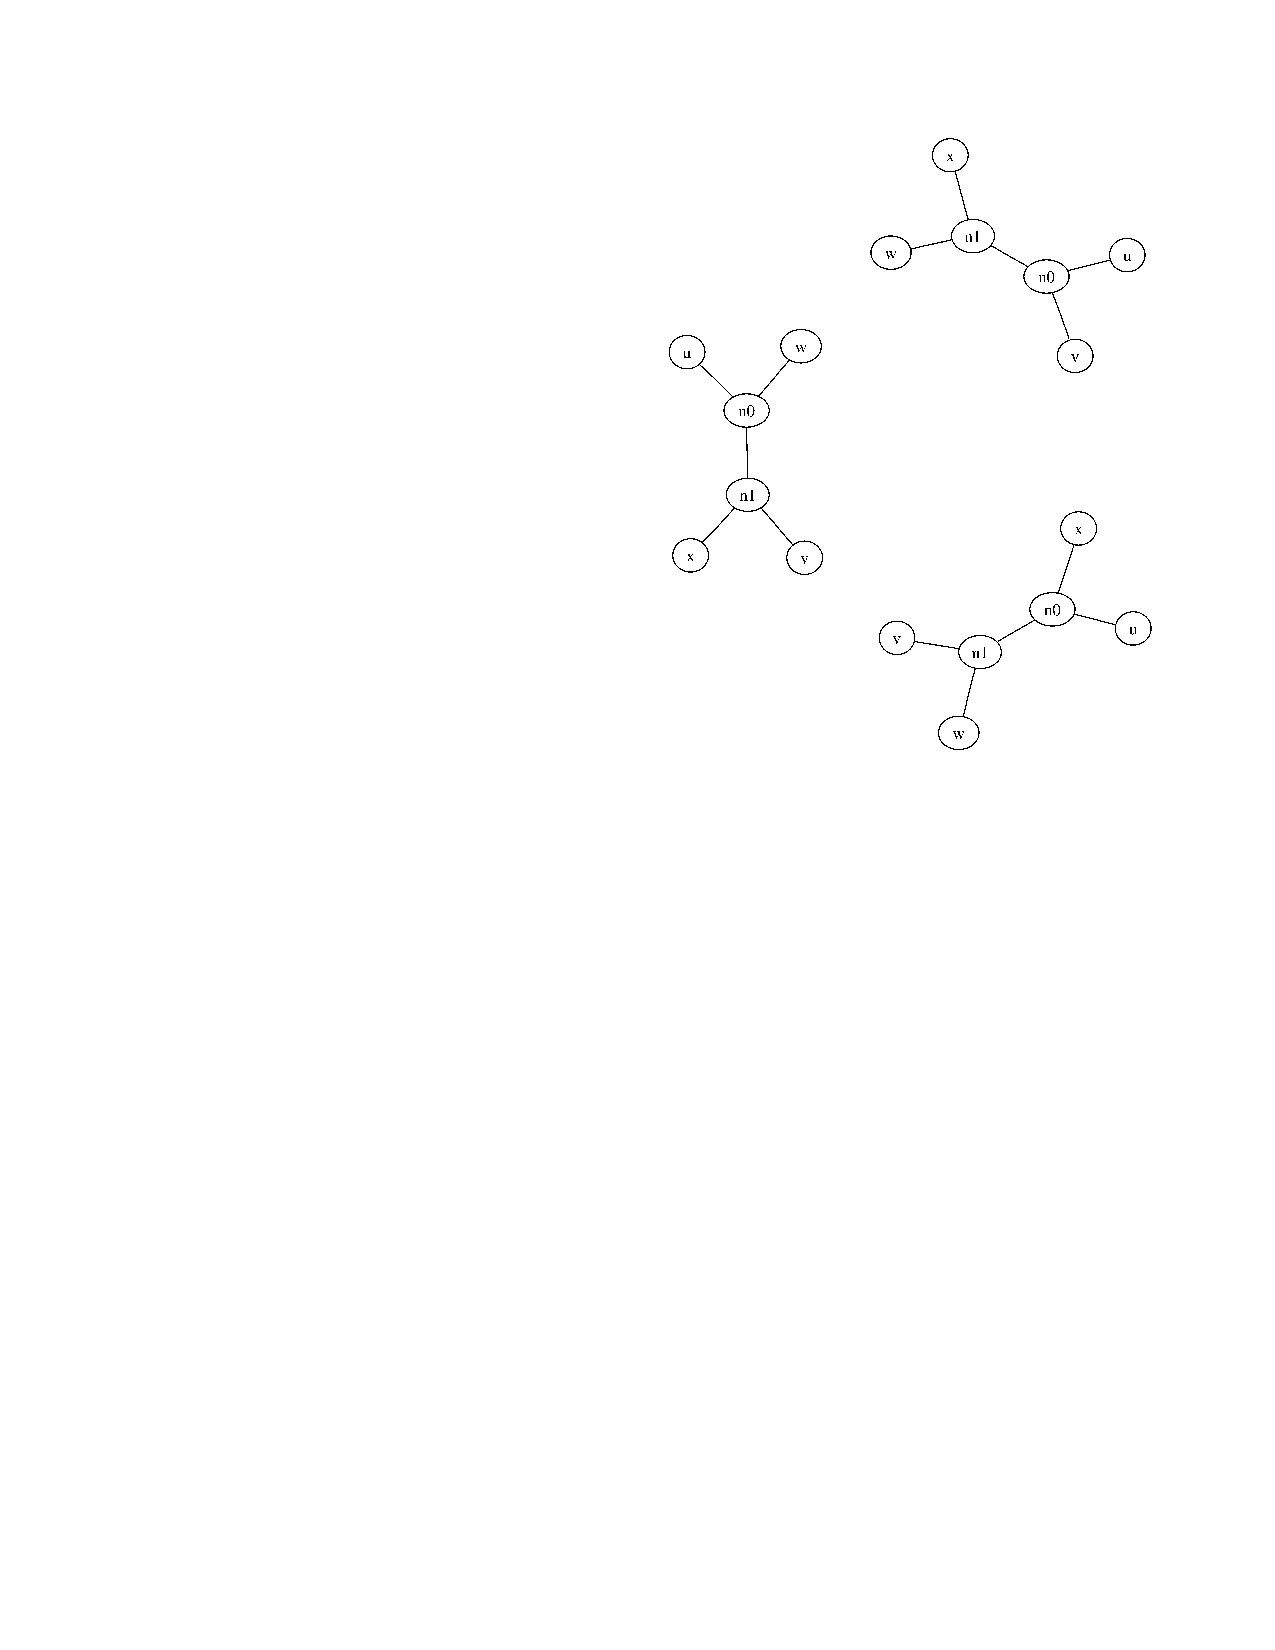
\includegraphics{img/ternary-tree}
      \caption{\emph{Kolme mahdollista nelikkotopologiaa}
      \cite{CV05}}
      \label{fig:ternary-tree}
    \end{figure}



    Jokaista määrättyä puuta $T$ ja jokaista lapsisolmumerkin ryhmää $\{u,v,w,x\}$ kohden sanomme että $T$ on johdonmukainen $uv|wx$:n kanssa, joss polku $u$:sta $v$:hen ei risteä polun $w$:stä $x$:än kanssa.

    Voimme kuvitella isomman puun rakentuvan monesta pienemmästä nelikkotopologiasta. Yleisesit nelikkomenetelmän tarkoitus on löytää tai approksimoida mahdollisimman lähelle puu joka sisältää maksimaalisen määrän johdonmukaisia nelikkotopologioita määrtystä joukosta $Q$. Tätä kutsutaan \emph{maksimi nelikkojohdonmukaisuudeksi} (MGC) \engl{maximum quartet consistency}

  %"minimum quartet tree cost" -> "pienin nelikkopuukustannus"

  %"quartet-based tree construction" -> "nelikkopohjainen puunrakennus"
  \paragraph{TODO} % (fold)
    \begin{itemize}
      \item puun rakentaminen etäisyysmatriisista
      \item Puun operaatiot
      \item normalisoitu puun hyötyarvo $S(T)$
      \item Satunnaisuuden käyttö tarkistusiteraatiossa parhaan puun approksimoimiseksi
    \end{itemize}
    % subsection nelikkomenetelma (end)

    Empiirisesti on havaittu, että hierarkkinen klusterointi toimii parhaiten pienille joukoille dataa (alle 25 objektia) ja sen toimivuus laskee huomattavasti isoille joukoille (yli 40 objektia). Yleinen ratkaisu isojen joukkojen hierarkkiseen klusterointiin on että, ensiksi klusteroidaan epähierarkkisesti ja sitten klusteroimalla hierarkkisesti tästä saatavat klusterit.
    \subsection{Tuloksia} % (fold)
    \label{sub:tuloksia}
      \paragraph{TODO} % (fold)
      \begin{itemize}
        \item Musiikin genrepuu
        \item Musiikin pieni vertaus
        \item Musiikin keskikokoinen vertaus
        \item Musiikin suuri vertaus
      \end{itemize}

    % subsection tuloksia (end)
  % section klusterointi (end)

\section{Algoritmin ongelmat ja ominaisuudet} % (fold)
\label{sec:algoritmin_ongelmat_ja_ominaisuudet}
    \begin{figure}[tb]
      \immediate\write18{pdfcrop img/noise-001}
      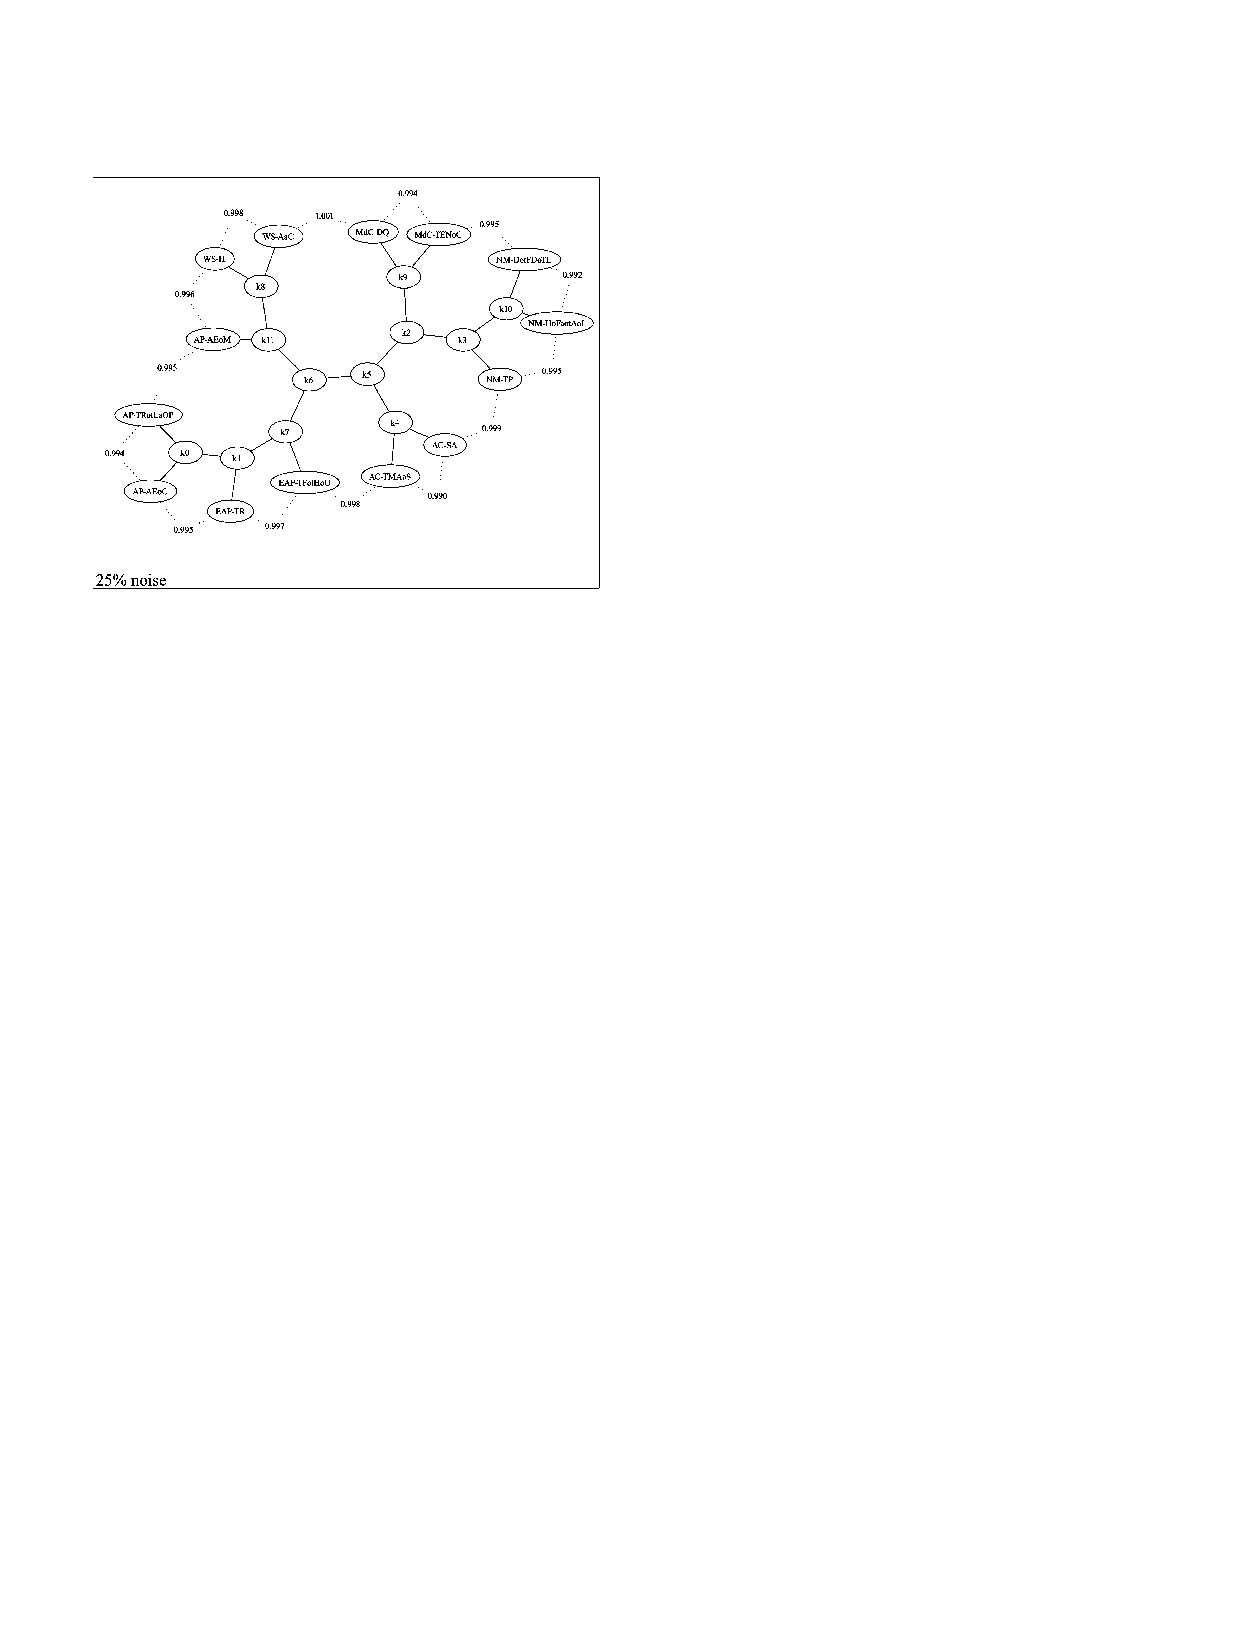
\includegraphics{img/noise-001}
      \caption{\emph{Normalisoitujen pakkausetäisyyksien pohjalta klusteroituja kirjoja eri kirjoittajilta kun tiedostoihin on lisätty 25\% kohinaa. Merkinnät ovat kirjailijan nimikirjaimet: AC = Agatha Christie, AP = Alexander Pope, EAP = Edgar Allan Poe, WS = William Shakespeare ja NM = Niccolo Machiavelli.}
      % TODO: The quality of the clustering degrades slowly due to the linear growth of the average distortion.
      \cite{4167725}}
      \label{fig:noise-001}
    \end{figure}
    \begin{figure}[tb]
      \immediate\write18{pdfcrop img/noise-002}
      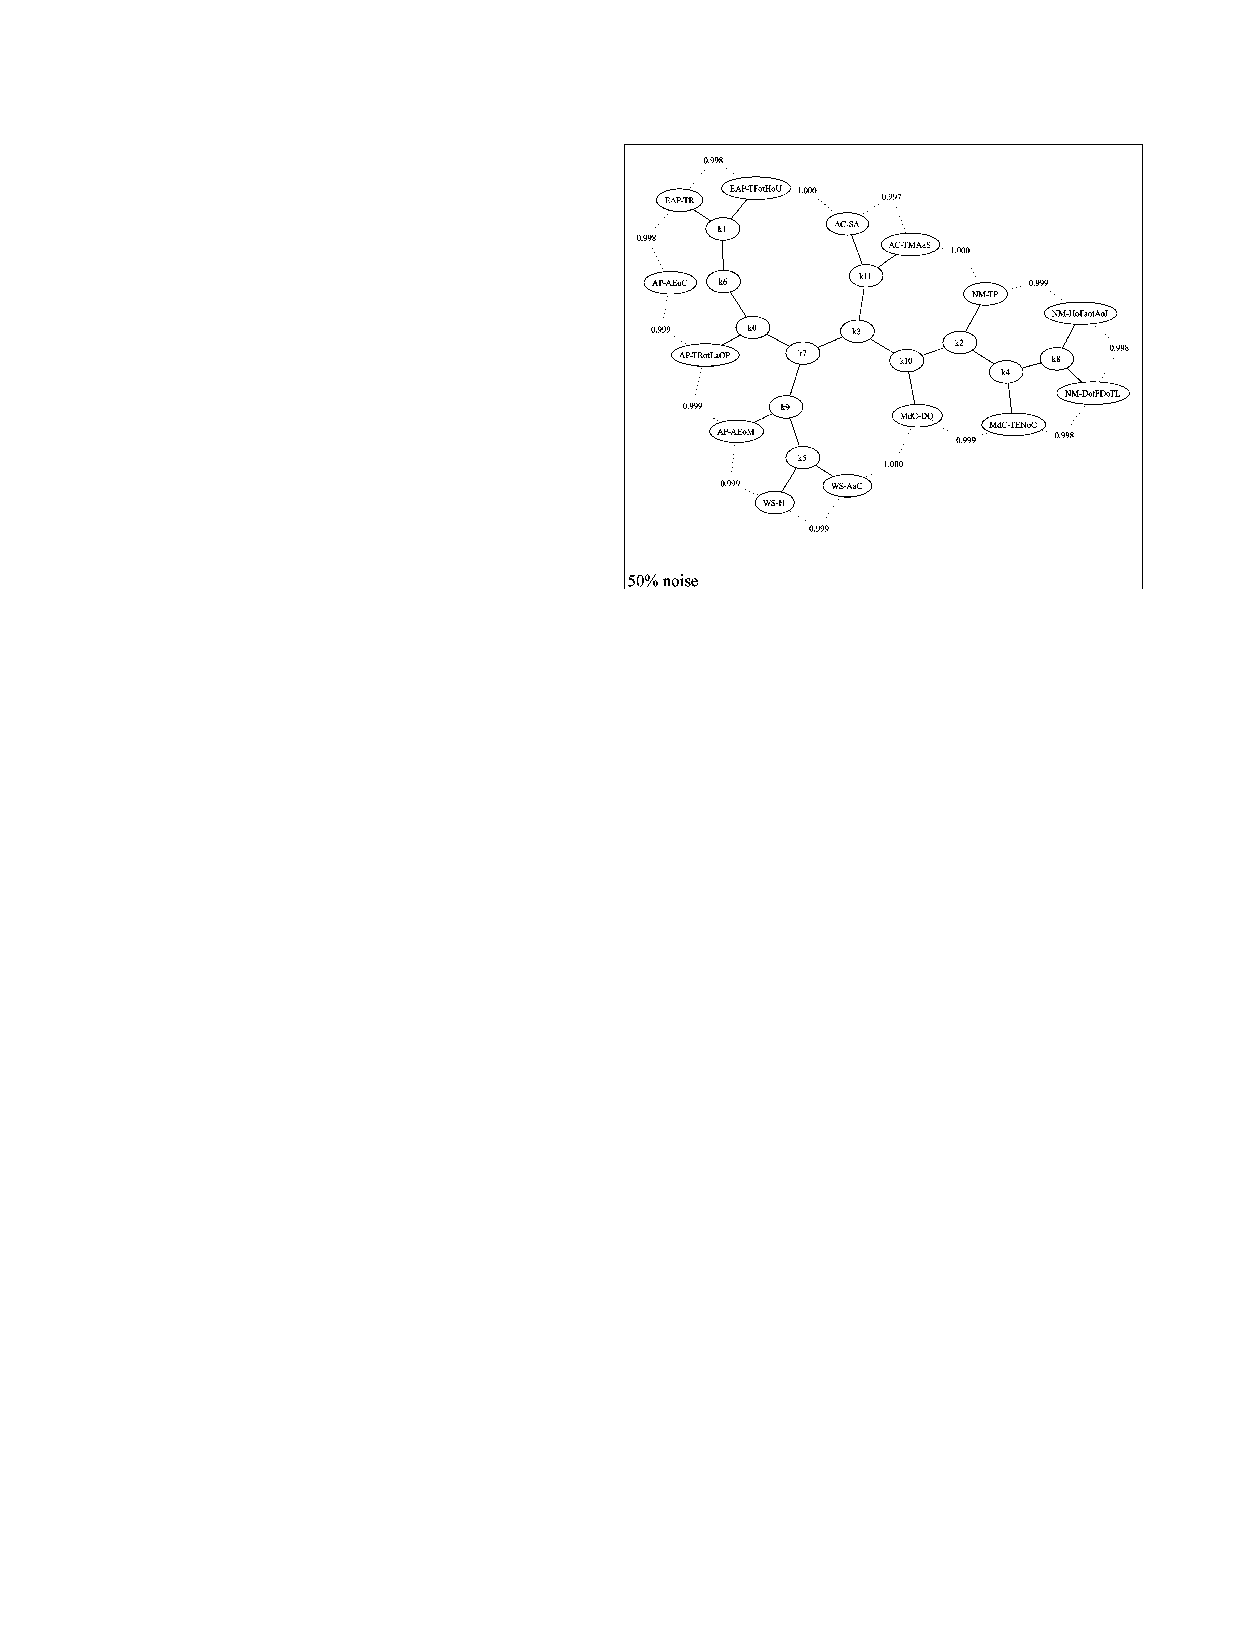
\includegraphics{img/noise-002}
      \caption{\emph{Normalisoitujen pakkausetäisyyksien pohjalta klusteroituja kirjoja eri kirjoittajilta kun tiedostoihin on lisätty 50\% kohinaa. Merkinnät vastaavat kuvaa \ref{fig:noise-001}.}
      % TODO: The quality of the clustering degrades slowly due to the linear growth of the average distortion.
      \cite{4167725}}
      \label{fig:noise-002}
    \end{figure}
    \begin{figure}[tb]
      \immediate\write18{pdfcrop img/noise-003}
      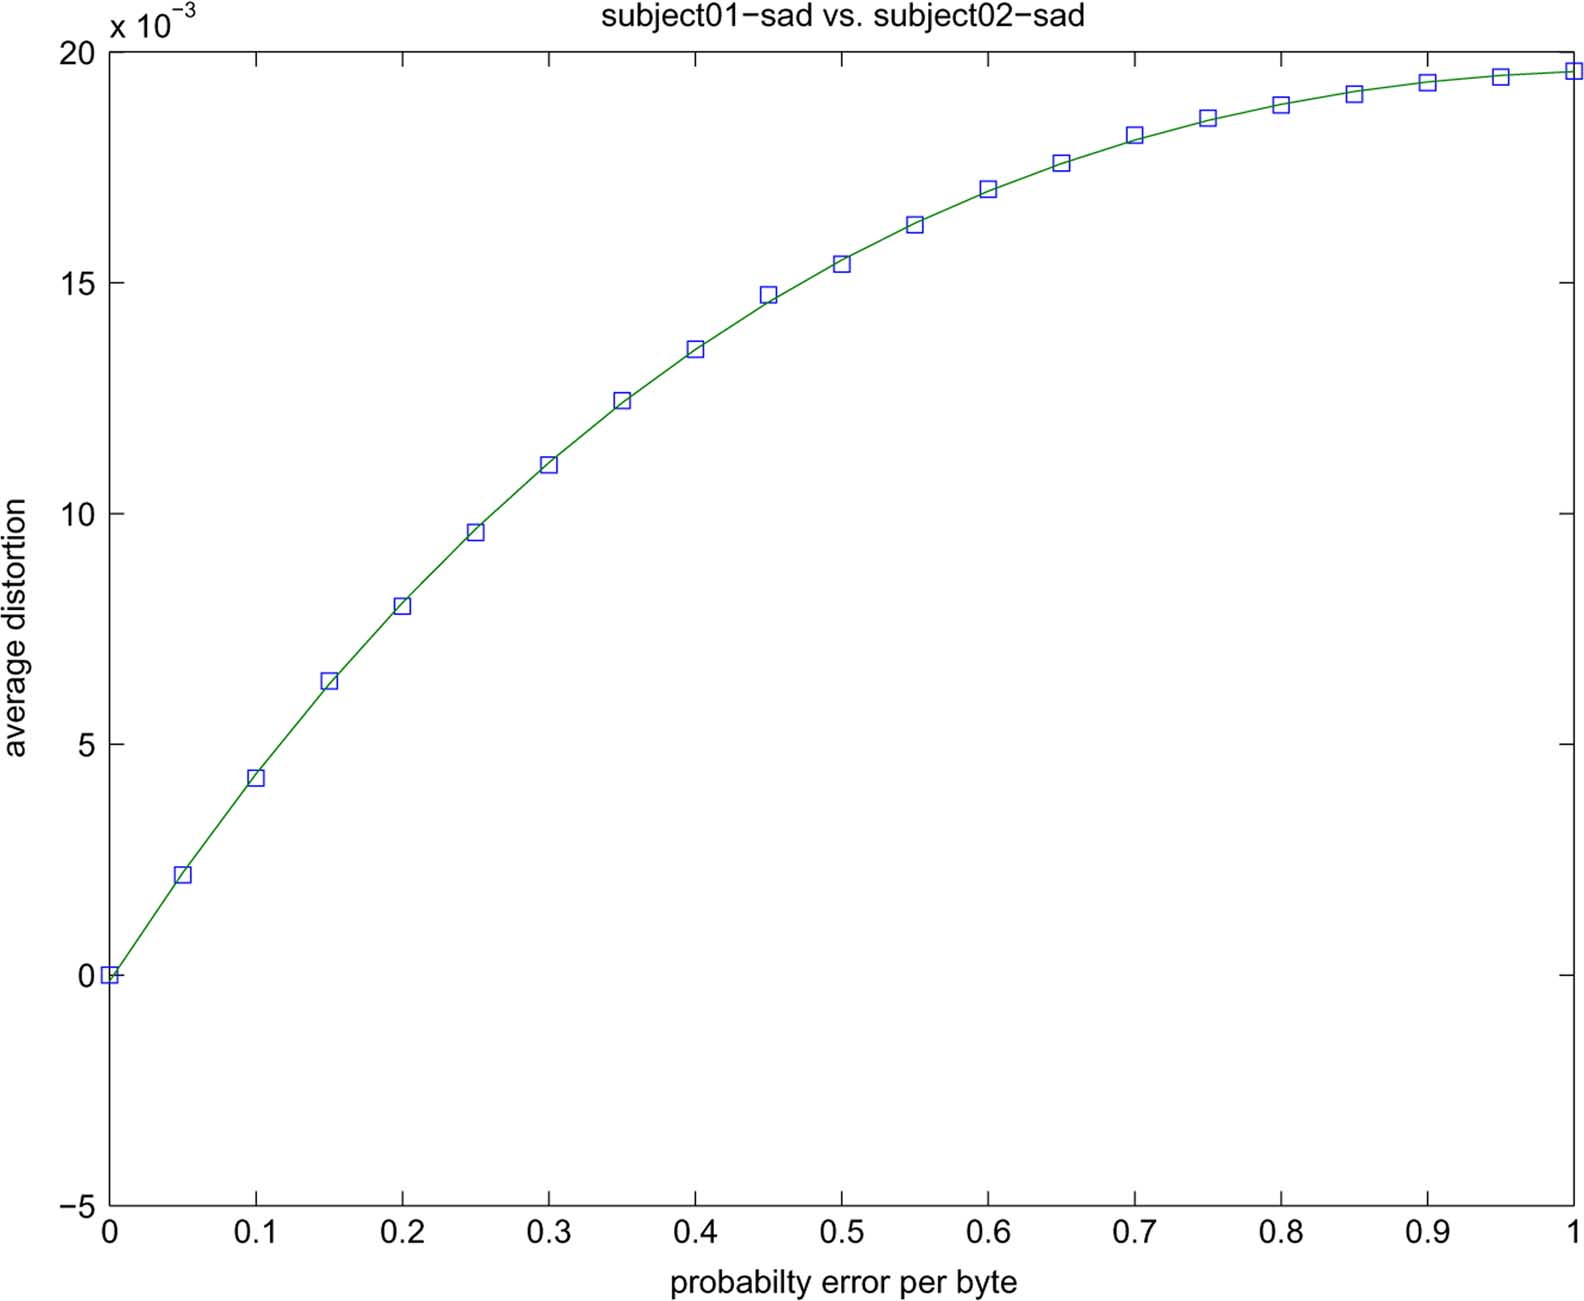
\includegraphics{img/noise-003}
      \caption{\emph{Normalisoitujen pakkausetäisyyksien pohjalta klusteroituja kirjoja eri kirjoittajilta kun tiedostoihin on lisätty 75\% kohinaa. Merkinnät vastaavat kuvaa \ref{fig:noise-001}.}
      % TODO: The quality of the clustering degrades slowly due to the linear growth of the average distortion.
      \cite{4167725}}
      \label{fig:noise-003}
    \end{figure}
  \subsection{Kohinansietokyky} % (fold)
  \label{sub:kohinansietokyky}

  % TODO: Approximoi differentiaaliyhtälöllä
    Kun NCD:tä käytetään kahteen eri tiedostoon toista näistä voi pitää kohinallisena versiona ensimmäisestä.
    Kohinan lisääminen progressiivisesti tiedostoon voi tuottaa tietoa mittarista \engl{measure} itsestään.
    Kuvissa \ref{fig:noise-001}, \ref{fig:noise-002}, \ref{fig:noise-003} on ternääripuut kirjojen klusteroinnista, kun objekteihin on lisätty kohinaa. Kuvissa merkitty kohinan osuus.
    Tämän vastaavuuden perusteella voimme tehdä teoreettisen päätelmän odotetusta kohinan lisäämisen vaikutuksesta algoritmiin, mikä selittää miksi NCD voi saada suurempia arvoja kuin $1$ joissain tapauksissa. \cite{4167725}


  % subsection kohinansietokyky (end)

  \subsection{Pakkaajan valinta} % (fold)
  \label{sub:pakkaajan_valinta}

    \begin{figure}[tb]
      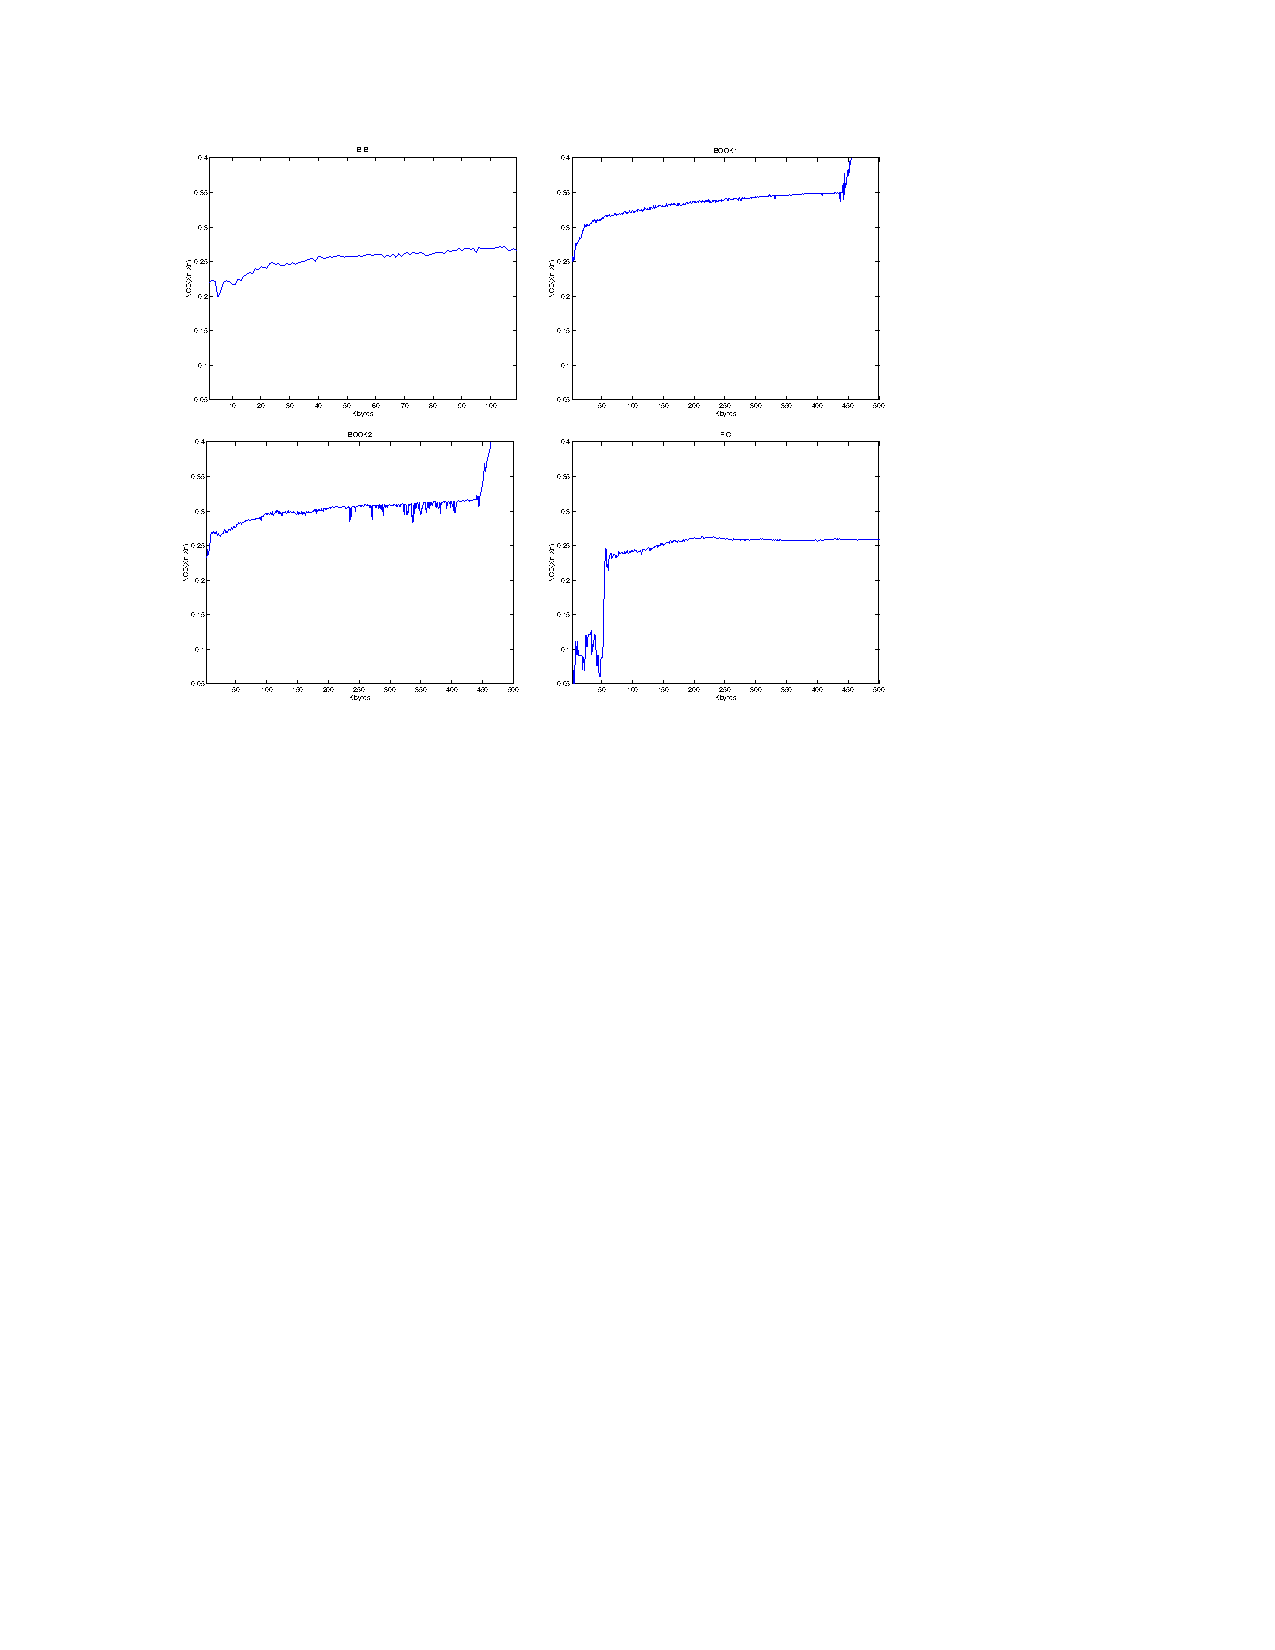
\includegraphics[width=\textwidth]{img/bzip2-best}
      \caption{\emph{Normalisoidut pakkausetäisyydet ensimmäisestä $n$ tavusta, neljälle tiedostolle Calgary Corpus -kokoelmasta, käyttäen \textbf{bzip2} pakkaajaa asetuksella `--best'. Tiedostot vertailtiin itsensä kanssa.} \cite{cebrian2005common}}
      \label{fig:bzip2-best}
    \end{figure}
    \begin{figure}[tb]
      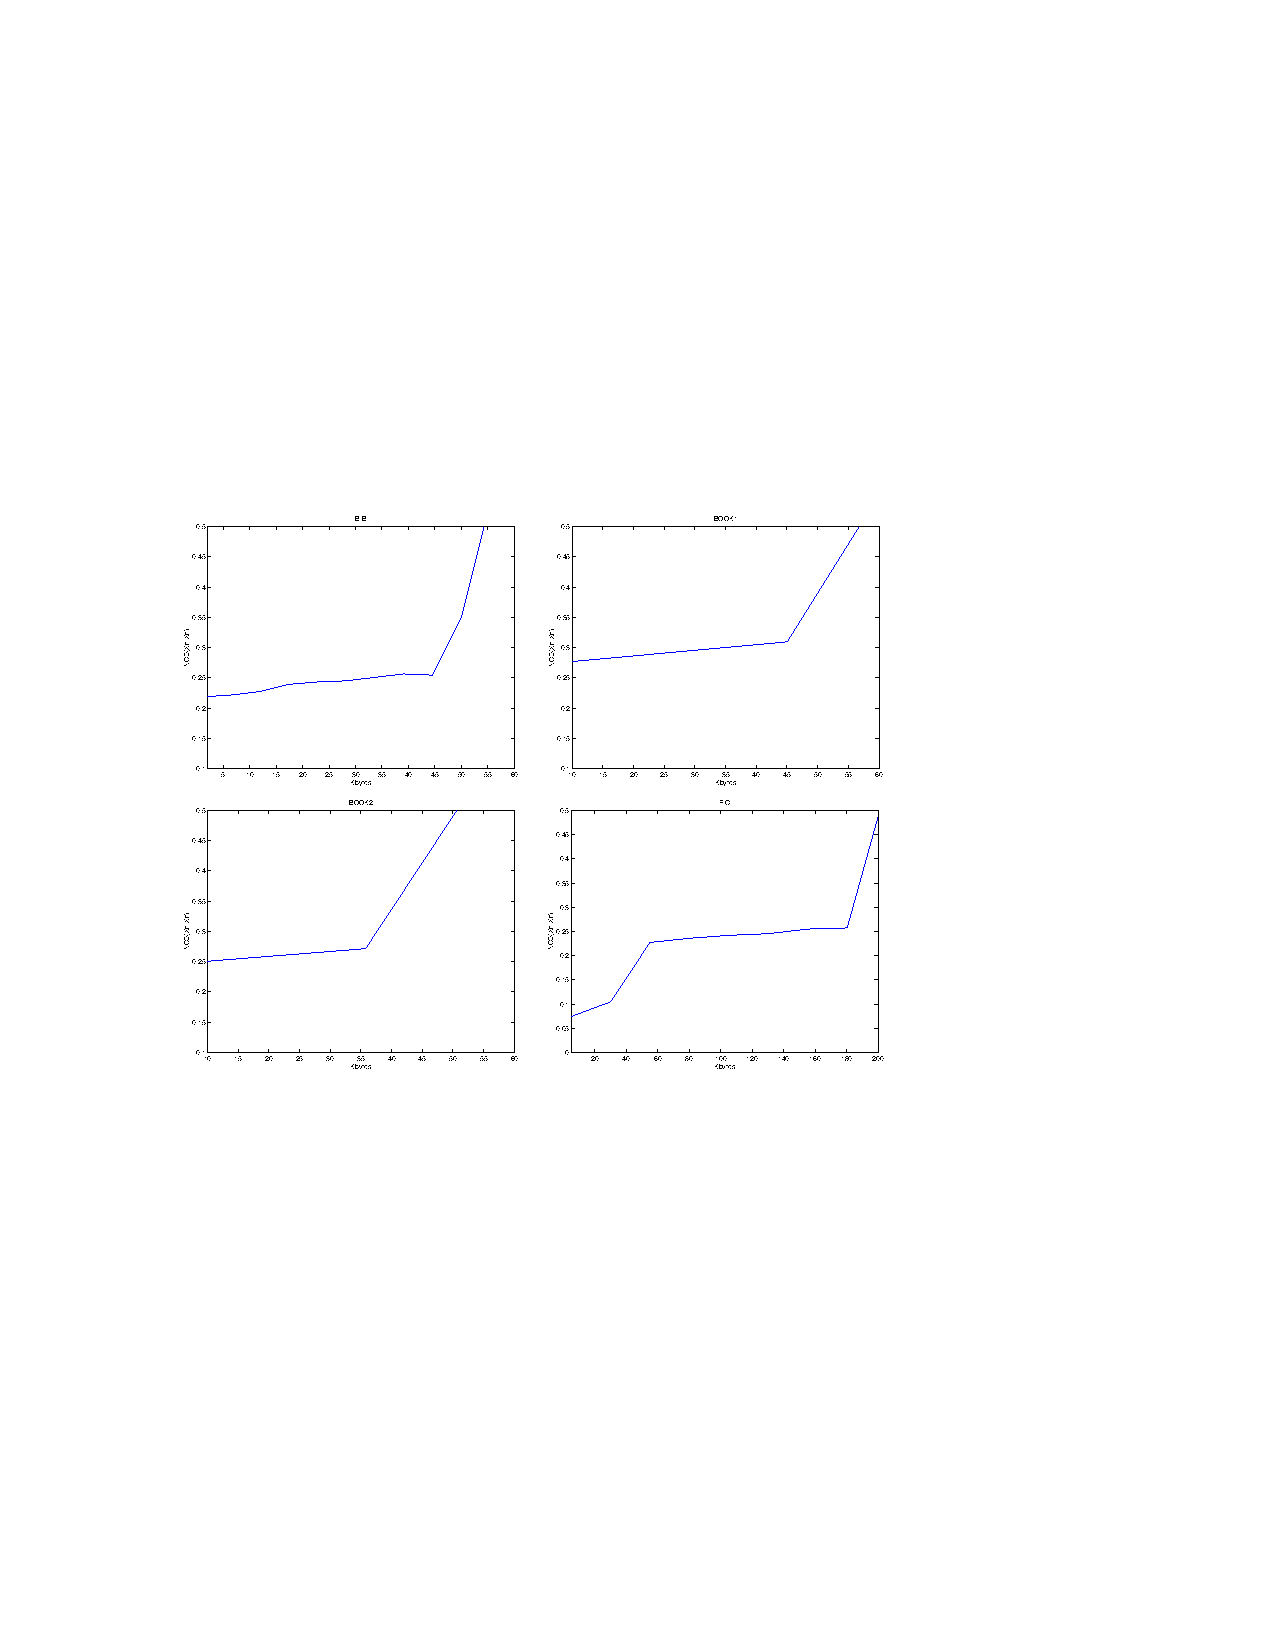
\includegraphics[width=\textwidth]{img/bzip2-fast}
      \caption{\emph{Normalisoidut pakkausetäisyydet ensimmäisestä $n$ tavusta, neljälle tiedostolle Calgary Corpus -kokoelmasta, käyttäen \textbf{bzip2} pakkaajaa asetuksella `--fast'. Tiedostot vertailtiin itsensä kanssa.} \cite{cebrian2005common}}
      \label{fig:bzip2-fast}
    \end{figure}
    \begin{figure}[tb]
      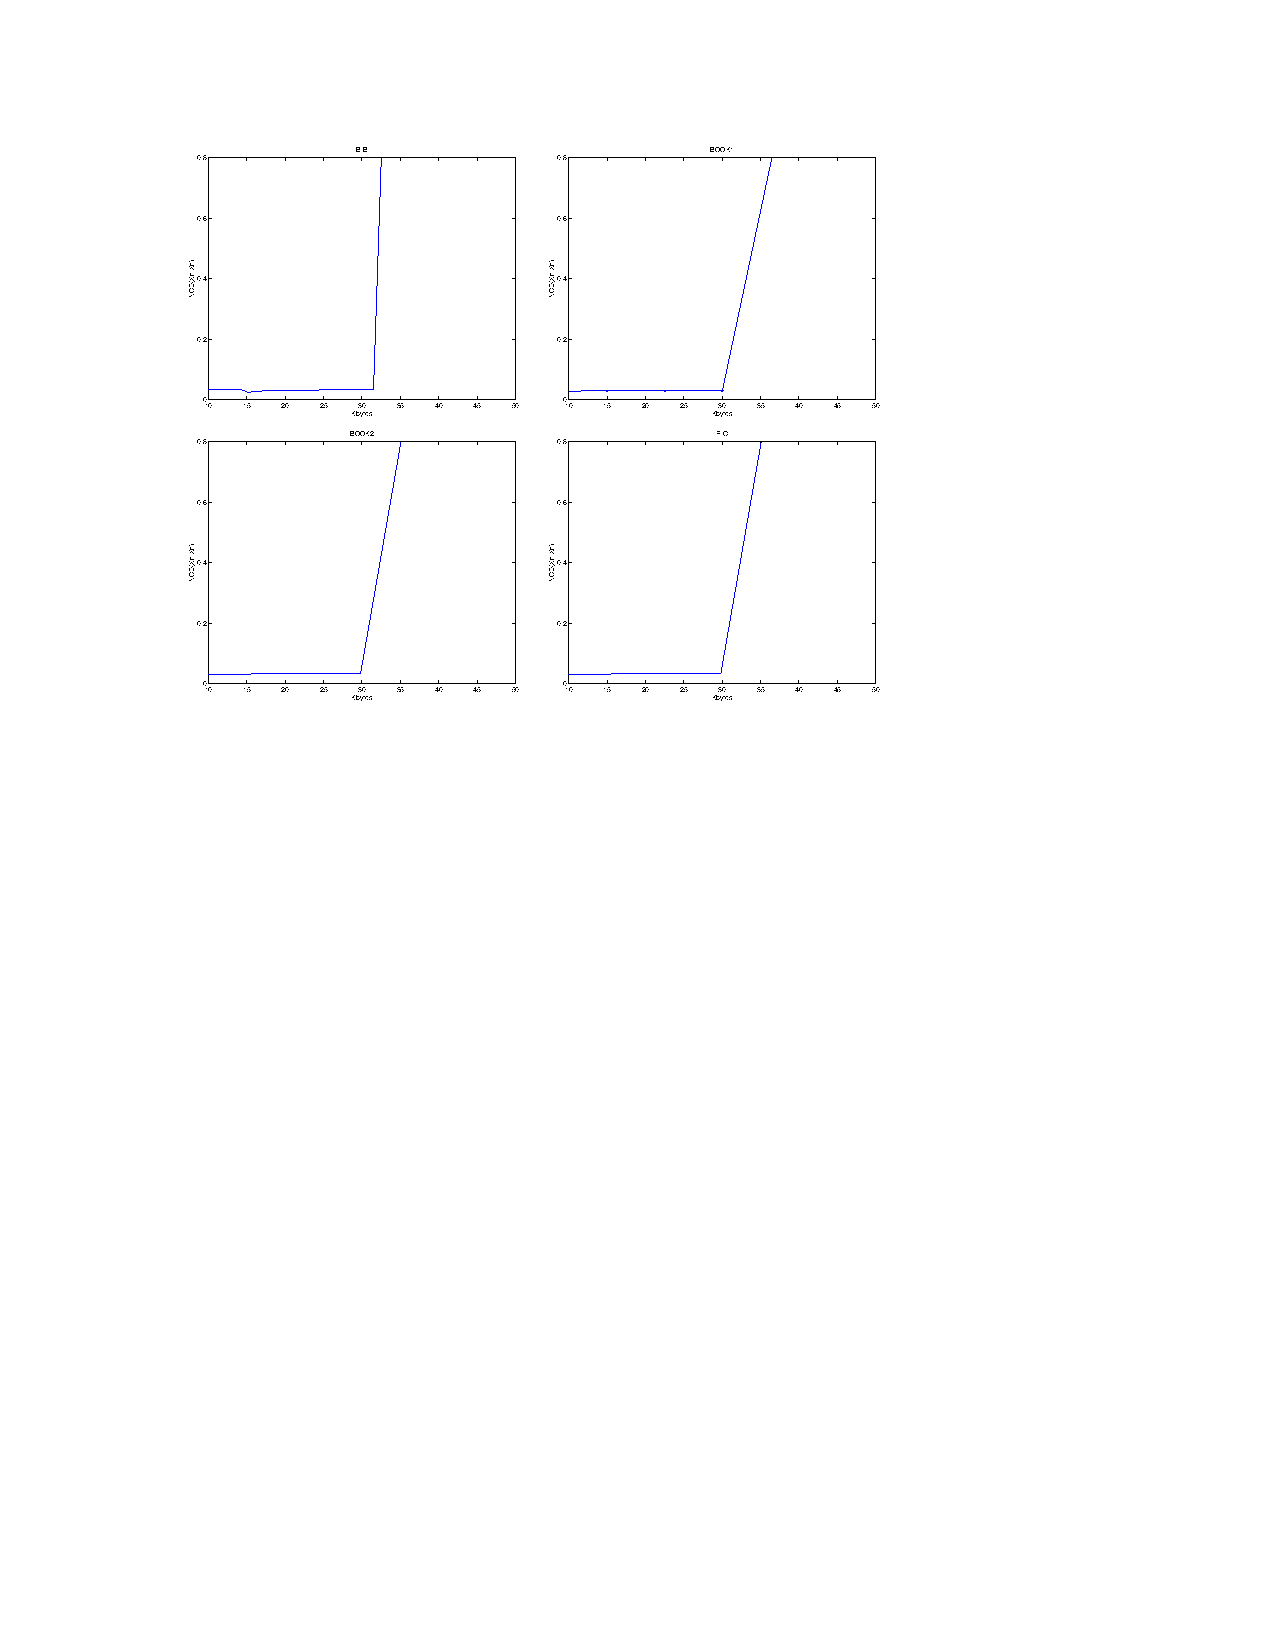
\includegraphics[width=\textwidth]{img/gzip-best}
      \caption{\emph{Normalisoidut pakkausetäisyydet ensimmäisestä $n$ tavusta, neljälle tiedostolle Calgary Corpus -kokoelmasta, käyttäen \textbf{gzip} pakkaajaa asetuksella `--best'. Tiedostot vertailtiin itsensä kanssa.} \cite{cebrian2005common}}
      \label{fig:gzip-best}
    \end{figure}
    \begin{figure}[tb]
        \immediate\write18{pdfcrop img/ppmz}
      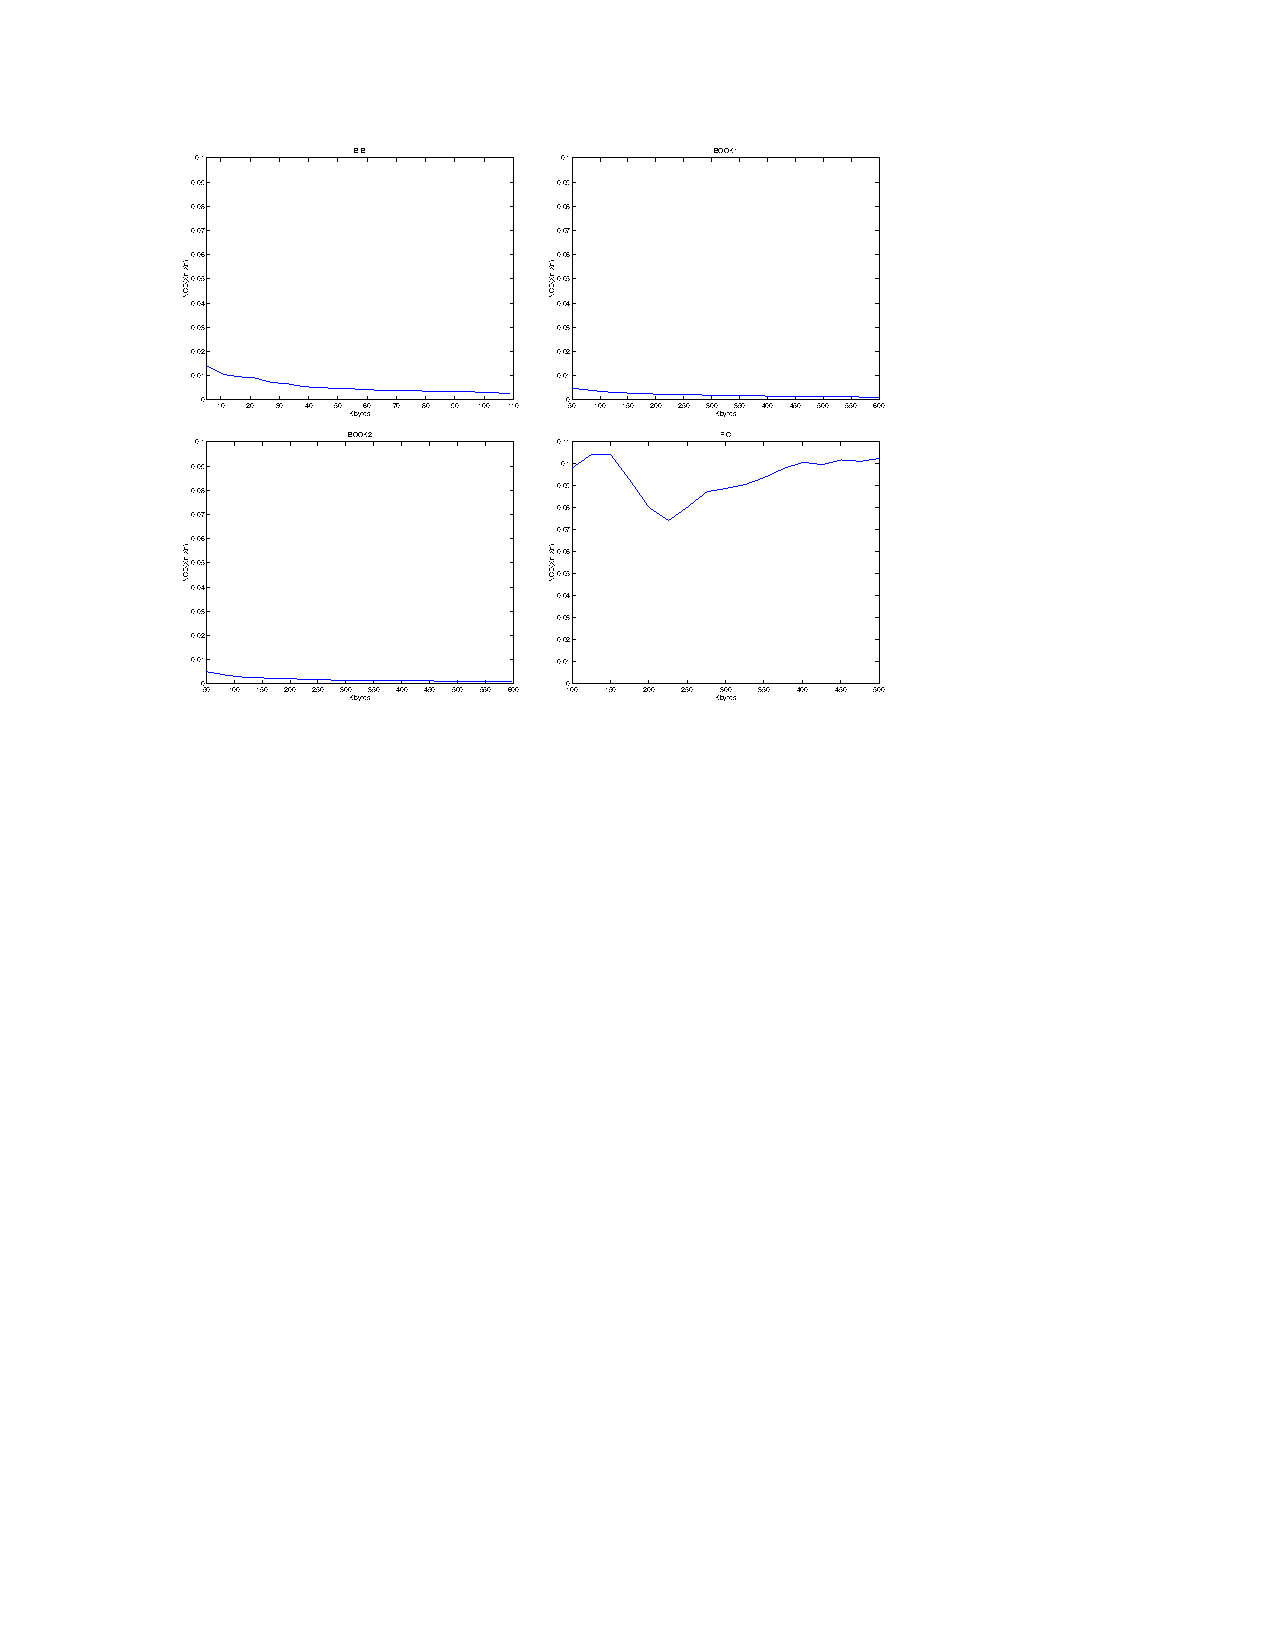
\includegraphics{img/ppmz}
      \caption{\emph{Normalisoidut pakkausetäisyydet ensimmäisestä $n$ tavusta, neljälle tiedostolle Calgary Corpus -kokoelmasta, käyttäen \textbf{PPMZ} pakkaajaa. Tiedostot vertailtiin itsensä kanssa.} \cite{cebrian2005common}}
      \label{fig:ppmz}
    \end{figure}
    \iffalse
    \fi
      Paperissa \cite{cebrian2005common} on osoitettu että, pakkaaja jota käytetään NCD:m laskemiseen ei ole idempotentti (\ref{idempotency}) kaikissa tapauksissa, koska objektien koko ja pakkaajan ikkunakoko vääristävät etäisyyksiä ja täten aiheuttavat poikkeuksia samankaltaisuuksissa. Yhteyttä etäisyyden tarkkuudesta ja objektien koosta on analysoitu monella tunnetulla pakkaajalla ja erityisesti seuraavilla kolmella:  \emph{bzip2}, \emph{gzip} ja \emph{PPMZ}.

      Vertailussa käytettiin Cilibrasin toteuttamaa CompLearn -työkalua \cite{complearn}, josta löytyy bzip2 ja gzip pakkaajat.
      Aineistona käytettiin tunnettua Calgary Corpus -kokoelmaa \cite{calgarycorpus}, joka on 18 tiedoston kokoelma jolla mitataan pakkausalgoritmien suorituskykyä.
      Kokoelmassa on 9 eri tyyppistä tiedostoa, jotta voidaan saada laaja näkemys pakkausalgoritmin toiminnasta.
      Mukana muun muassa on kuva, kirjoja, artikkeleita, lähdekoodia ja tietokoneohjelmia.

      Kaikkia vertailun objekteja käsitellään merkkijonoina, jotka koostuvat tavuista.
      Jotta voitiin todeta pakkaajan idempotenssin (\ref{idempotency}) pätevyys, kaikki objektit vertailtiin itsensä kanssa.

      \paragraph{bzip2} % (fold)
      \label{par:bzip2}
        Kuvassa \ref{fig:bzip2-best} huomataan että $NCD(x,x)$ on väliltä $0.2$ ja $0.3$, kun tiedostojen koko on sopiva bzip2 pakkaajalle, kun taas arvo on väliltä $0.25$ ja $0.9$ kun tiedostokoko ei ole enää sopiva.
        Rajoittava tekijä bzip2 pakkaajassa on tälle määriteltävä lohkokoko \engl{block size}, joka on oletusarvoisesti 900 kilotavua, eli jos pakattavan tiedoston koko on tätä suurempi niin se pilkotaan alle 900 kilotavun kokoisiksi palasiksi ennen pakkausta.
        Tällaisesta pilkkomisesta aiheutuu se, ettei eri osien välillä pysty enää pakkaamaan samankaltaisuuksia ja täten pakattu koko ei ole paras mahdollinen.
        Tämä näkyy hyvin kuvassa \ref{fig:bzip2-fast}, jossa lohkokoko on huomattavasti pienempi kuin 900 kilotavua ja täten NCD:n arvot nousevat hyvin pienillä tiedostoilla jo korkealle.
      % paragraph bzip2 (end)

      \paragraph{gzip} % (fold)
      \label{par:gzip}
        Kuva \ref{fig:gzip-best} osoittaa että $NCD(x,x)$ on väliltä $0.0$ ja $0.1$ kun tiedostokoko on sopiva gzip pakkaajalle, ja kun tiedostokoko on liian suuri niin arvot nousevat jopa yli $1$.
        Vastaavanlaisesti kuin bzip2 pakkaajassa on rajoittavana tekijänä lohkokoko, on gzip pakkaajassa liukuva ikkuna \engl{sliding window} ja eteenpäinkatseluikkuna \engl{lookahead window}.
        Liukuva ikkuna on puskuri jossa säilötään $n$ viimeisintä merkkiä, jossa $n$ on liukuvan ikkunan koko.
        Eteenpäinkatseluikkuna taas on puskuri jossa on $m$ tulevaa merkkiä, jossa $m$ on eteenpäinkatseluikkunan koko.

        Nämä ikkunakoot aiheuttavat sen, että parhaimmallakin asetuksella gzip kykenee pakkaamaan tehokkaasti ainoastaan enintään 64 kilotavua olevia tiedostoja.
      % paragraph gzip (end)

      Mikä tahansa samankaltaisuusetäisyys olisi pitänyt arvoltaan olla $0$ tai hyvin lähellä sitä, kun vertaillaan identtisiä objekteja.
      Pakkaajien vertailussa kerätyt empiiriset havainnot osoittavat että objektien koko vääristää NCD:n tulosta, riippumatta datan tyypistä (kirja, artikkeli, kuva, jne.)
      Siksi suositellaan PPMZ pakkaajan käyttöä kun halutaan klusteroida objekteja NCD:lla \cite{cebrian2005common}.
      Muitten pakkaajien käyttö on suositeltavaa ainoastaan, jos pyritään nopeuteen tai jos tiedostojen kokojen summa on pienempi kuin pakkaajan käyttämä rajoite (lohkokoko, ikkunakoko).

  % subsection pakkaajan_valinta (end)
% section algoritmin_ongelmat_ja_ominaisuudet (end)

\section{Google-samankaltaisuusetäisyys} % (fold)
  \label{sec:google_samankaltaisuusetaisyys}

    Internetin kasvu on houkutellut miljoonia käyttäjiä luomaan miljardeja internetsivuja, jotka ovat sisällöltään ja piirteiltään hyvin vaihtelevia.
    Suunnaton tiedon määrä miltei mistä tahansa aiheesta tekee siitä mahdollisen, että ääripäät kumoutuvat ja täten suurin osa tai keskiverto on merkitsevä heikkolaatuisena approksimaationa.
    Täten on kehitetty yleinen metodi hyödyntämään tätä matalalaatuista tietoa, jota saa ilmaiseksi Internetistä.
    Tämä tietovarasto on kaikille käytettävissä käyttäen mitä tahansa hakukonetta, joka pystyy palauttamaan yhteenlasketun sivulukumääräarvion, kuten Google.

    Google-samankaltaisuusetäisyys (\emph{GSD}) on hyvin vahvasti verrattavissa Normalisoituun pakkausetäisyyteen (kts. \ref{sub:normalisoitu_pakkausetaisyys},) sillä kummatkin algoritmit perustuvat samoihin tekniikoihin, kuten Kolmogorov-kompleksisuuteen (kts. \ref{sub:kolmogorov_kompleksisuus}) ja Normalisoituun informaatioetäisyyteen (\ref{sub:normalisoitu_informaatioetaisyys}).
    Eroavaisuuksia esiintyy siinä, mitä nämä kaksi algoritmia käyttävät samankaltaisuuden arvioimiseksi.
    Siinä missä NCD pakkaa ja vertaa sisältöä toisiinsa, niin GSD vertaa asioitten nimiä esiintymistiheyteen. \cite{cilibrasi2007google}

    \subsection{Käytännön esimerkki} % (fold)
    \label{sub:kaytannon_esimerkki}
      GSD muodostetaan siten että haetaan ensiksi yhdellä hakutermillä, sitten toisella ja sen jälkeen kummallakin yhdessä.
      Hakujen lukumäärät vertaillaan keskenään ja normalisoidaan ja tästä saadaan samankaltaisuusetäisyys.

      Paperissa \cite{cilibrasi2007google} käytettiin hakusanoja ``horse'' ja ``rider'' esimerkkinä ja vuonna 2007 tuloksena oli $NGD(horse, rider) \approx 0.443$.
      Toistimme kyseisen haun 13.11.2013 ja tuloksena oli $NGD(horse, rider) \approx 0.233$.
      Arvojen suurta eroa on vaikea selvittää ilman laajempaa tutkimusta, mutta vaikuttavia tekoja voi olla epäselvyys tarkasta lukumäärästä Googlen indeksoimista sivuista.

    % subsection kaytannon_esimerkki (end)

    \subsection{Hakukoneet samankaltaisuuden mittaamisessa} % (fold)
    \label{sub:hakukoneet_samankaltaisuuden_mittaamisessa}

    Googlen indeksoitujen internetsivujen määrä on kasvanut suunnattomaksi ja mikä tahansa yleinen hakutermi esiintyy miljoonilla internetsivulla. Internetin sisällöntuottajiakin on suunnaton määrä ja voidaan olettaa näiden olevan erittäin kuvaava otanta isosta osasta ihmiskuntaa.
    Tämän perusteella voidaan argumentoida että, Google-haun frekvenssi on kuvaava approksimaatio todellisista relatiivisista frekvensseistä yhteiskunnassa.
    Frekvenssi on haun tuottamien osumien lukumäärän suhde kaikkien Googlen indeksoimien sivujen lukumäärään. \cite{cilibrasi2007google}

    % subsection hakukoneet_samankaltaisuuden_mittaamisessa (end)
    \subsection{Google-jakauma} % (fold)
    \label{sub:google_jakauma}
      Olkoon yksittäisten Google-hakujen joukko $S$.
      Jatkossa käytämme yksittäisten ja pareittaisten hakujen joukkoja $\{\{x,y\}:x,y \in S\}$.
      Olkoon joukko Googlen indeksoimia internetsivuja $\Omega$.
      Joukon $\Omega$ koko merkitään $M = |\Omega|$.
      Oletamme että jokaisella internetsivulla on yhtä todennäköistä palautua Google-hausta, eli todennäköisyys on $\frac{1}{\Omega}$.
      $\Omega$:n osajoukkoa kutsutaan \emph{tapahtumaksi}.
      Jokainen hakuehto $x$ määrittelee yksittäisen haun tapahtuman $\mathbf{x}\subseteq \Omega$, tämä on joukko internetsivuja joista löytyy $x$ kun suoritetaan Google-haku $x$:llä.
      Olkoon $L: \Omega \rightarrow [0,1]$ tasajakauman todennäköisyysfunktio.
      Tapahtuman $\mathbf{x}$ todennäköisyys on $L(\mathbf{x}) = \frac{|\mathbf{x}|}{M}$.
      Samoin toimii pareittain haun tapahtuma $\mathbf{x}\cap\mathbf{y}\subseteq\Omega$, jossa haetaan pareittain hakuehdoilla $x$ ja $y$.

      Kaikkien tapahtumien todennäköisyydet yhteensä on suurempi kuin $1$, koska tapahtumat menevät päällekkäin, joten tarvitaan normalisointia.
      $|S|$ on yksittäisten ja $\binom{|S|}{2}$ parittaisten hakujen tulosten lukumäärä.
      Määrittelemme
      \begin{align}
        N = \sum_{\{x,y\} \subseteq S} |x \cap y|,
      \end{align}
      yksittäisten ja parittaisten hakujen tulosten lukumäärä yhteensä.
      $N \geq M$, koska jokainen Googlen indeksoima internetsivu sisältää vähintään yhden hakusanan esiintymän. Toisaalta internetsivuilla ei keskivertona ole enempää kuin $\alpha$ hakutermiä, täten $N \leq \alpha{}M$.
      Määrittelemme
      \begin{align}
        g(x) = g(x,x),\, g(x,y) = L(\mathbf{x} \cap \mathbf{y})\frac{M}{N} = \frac{|\mathbf{x}\cap \mathbf{y}|}{N}.
      \end{align}
      Ja siten looginen seuraus on $\sum_{\{x,y\}\subseteq S} g(x,y) = 1$, eli $g$ määrittelee todennäköisyysjakauman.
    % subsection google_jakauma (end)

    \subsection{Google-samankaltaisuusetäisyys} % (fold)
    \label{sub:google_samankaltaisuusetaisyys}
      \emph{Normalisoitu Google-etäisyys} (\emph{NGD}) \engl{Normalized Google Distance}  voidaan määritellä seuraavasti,
      \begin{align}
        NGD(x,y) = \frac{max\{\log{f(x)},\log{f(y)}\}-\log{f(x,y)}}{\log{N}-min\{\log{f(x)},\log{f(y)}\}},
      \end{align}
      jossa $f(x)$ merkitsee internetsivujen lukumäärää, jotka sisältävät hakutermin $x$ ja $f(x,y)$ merkitsee samaa mutta sivuille jotka sisältävät termit $x$ ja $y$.
      Tämä normalisoitu Google-etäisyys on approksimaation normalisoidusta informaatioetäisyydestä \ref{sub:normalisoitu_informaatioetaisyys}.
      Käytännössä käytämme Googlen palauttamia sivujen lukumääriä frekvensseinä ja valitaan $N$.
      On huomattu että mikä tahansa järkevä arvo voidaan käyttää normalisoinnin arvona $N$.
      NGD:llä on seuraavat ominaisuudet, olettaen että valitaan parametri $N\geq{}M$:
      \begin{enumerate}
        \item NGD:n arvo on väliltä $0$ ja $\infty$ (mahdollisesti negatiivinen, jos Googlen lukumäärät ovat epäluotettavia ja täten $f(x,y) > max\{f(x),f(y)\}$)
        \begin{enumerate}
          \item Jos $x=y$ tai $x\neq{}y$, mutta frekvenssi on
          \[
            f(x) = f(y) = f(x,y) > 0,
          \]
          niin $NGD(x,y)=0$. Eli $x$ ja $y$ ovat Googlen kannalta samat.
          \item Jos frekvenssi $f(x)=0$, sitten jokaiselle hakutermille $y$ pätee $f(x,y)=0$. Tämän lisäksi pätee
          \[
            NGD(x,y)=\frac{\infty}{\infty}
          \]
          jonka määrittelemme tarkoittavan $1$.
        \end{enumerate}
        \item NGD on aina epänegatiivinen ja $NGD(x,x)=0$ kaikille $x$. Kaikille $x,y$ pätee $NGD(x,y)=NGD(y,x)$, toisin sanoen se on symmetrinen. NGD ei kuitenkaan ole metriikka, koska se ei täytä ehtoa $NGD(x,y) > 0$ kaikille $x\neq{}y$, eikä se myöskään toteuta metriikan kolmioepäyhtälö-ominaisuutta $NGD(x,z) \leq NGD(x,y) + NGD(y,z)$. \cite{cilibrasi2007google}
        \item NGD on \emph{invariantti skaalautuvuudessa} seuraavassa mielessä: Oletamme, että kun Googlen indeksoimien sivujen lukumäärä $N$ kasvaa, niin sivujen, jotka sisältävät annetun hakusanan, lukumäärä lähestyy määrättyä murto-osaa $N$:stä, ja niin myös sivujen lukumäärä, jotka sisältävät hakusanojen parin.
      \end{enumerate}
    % subsection google_samankaltaisuusetaisyys (end)

    \subsection{Hierarkkinen klusterointi} % (fold)
    \label{sub:klusterointi}
      Klusterointi normalisoidun Google-etäisyyden avulla onnistuu samanlailla kuin normalisoidulla pakkausetäisyydelläkin. Ensiksi koostetaan etäisyysmatriisi hakuehtojen pareittaisista NGD:n arvoista ja sitten nelikkomenetelmää \ref{sub:nelikkomenetelma} käyttäen rakennetaan \emph{juureton ternääripuu} \engl{unrooted ternary tree}.

      Esimerkkinä klusteroitiin 15, 1600-luvun hollantilaisten maalareitten, teosta.
      Kuvassa \ref{fig:dutch-paintings} on Rembrandtin, Steenin ja Bolin maalauksia ternääripuu-rakenteessa.
      Hakusanoina käytettiin ainoastaan maalausten koko nimiä. Seuraavaksi lista maalauksista ja teoksista

      \begin{itemize}
        \item \textbf{Rembrandt van Rijn:} \emph{Hendrickje slapend, Portrait of Maria Trip, Portrait of Johannes Wtenbogaert, The Stone Bridge, and The Prophetess Anna.}
        \item \textbf{Jan Steen:} \emph{Leiden Baker Arend Oostwaert, Keyzerswaert, Two Men Playing Backgammon, Woman at her Toilet, Prince’s Day, and The Merry Family.}
        \item \textbf{Ferdinand Bol:} \emph{Maria Rey, Consul Titus Manlius Torquatus, Swartenhout, and Venus and Adonis.}
      \end{itemize}

      Kuvassa \ref{fig:dutch-paintings} näemme, että suurin osa maalauksista ovat ryhmittyneet puun haaroihin taiteilijan mukaan. Rembrandtin maalaukset ovat oikealla, Steenin maalaukset vasemmalla ja Bolin maalaukset alhaalla. Muutama maalaus on hieman erillään taiteilijan ryhmittymästä ja nämä ovat Rembrandtin ``Hendrickje slapend'', Steenin ``Woman at her Toilet'' ja  Bolin ``Swartenhout'', joista viimeiset kaksi ovat luokiteltu väärän taiteilijan haaraan.

      \begin{figure}[tb]
        \immediate\write18{pdfcrop img/dutch-paintings}
        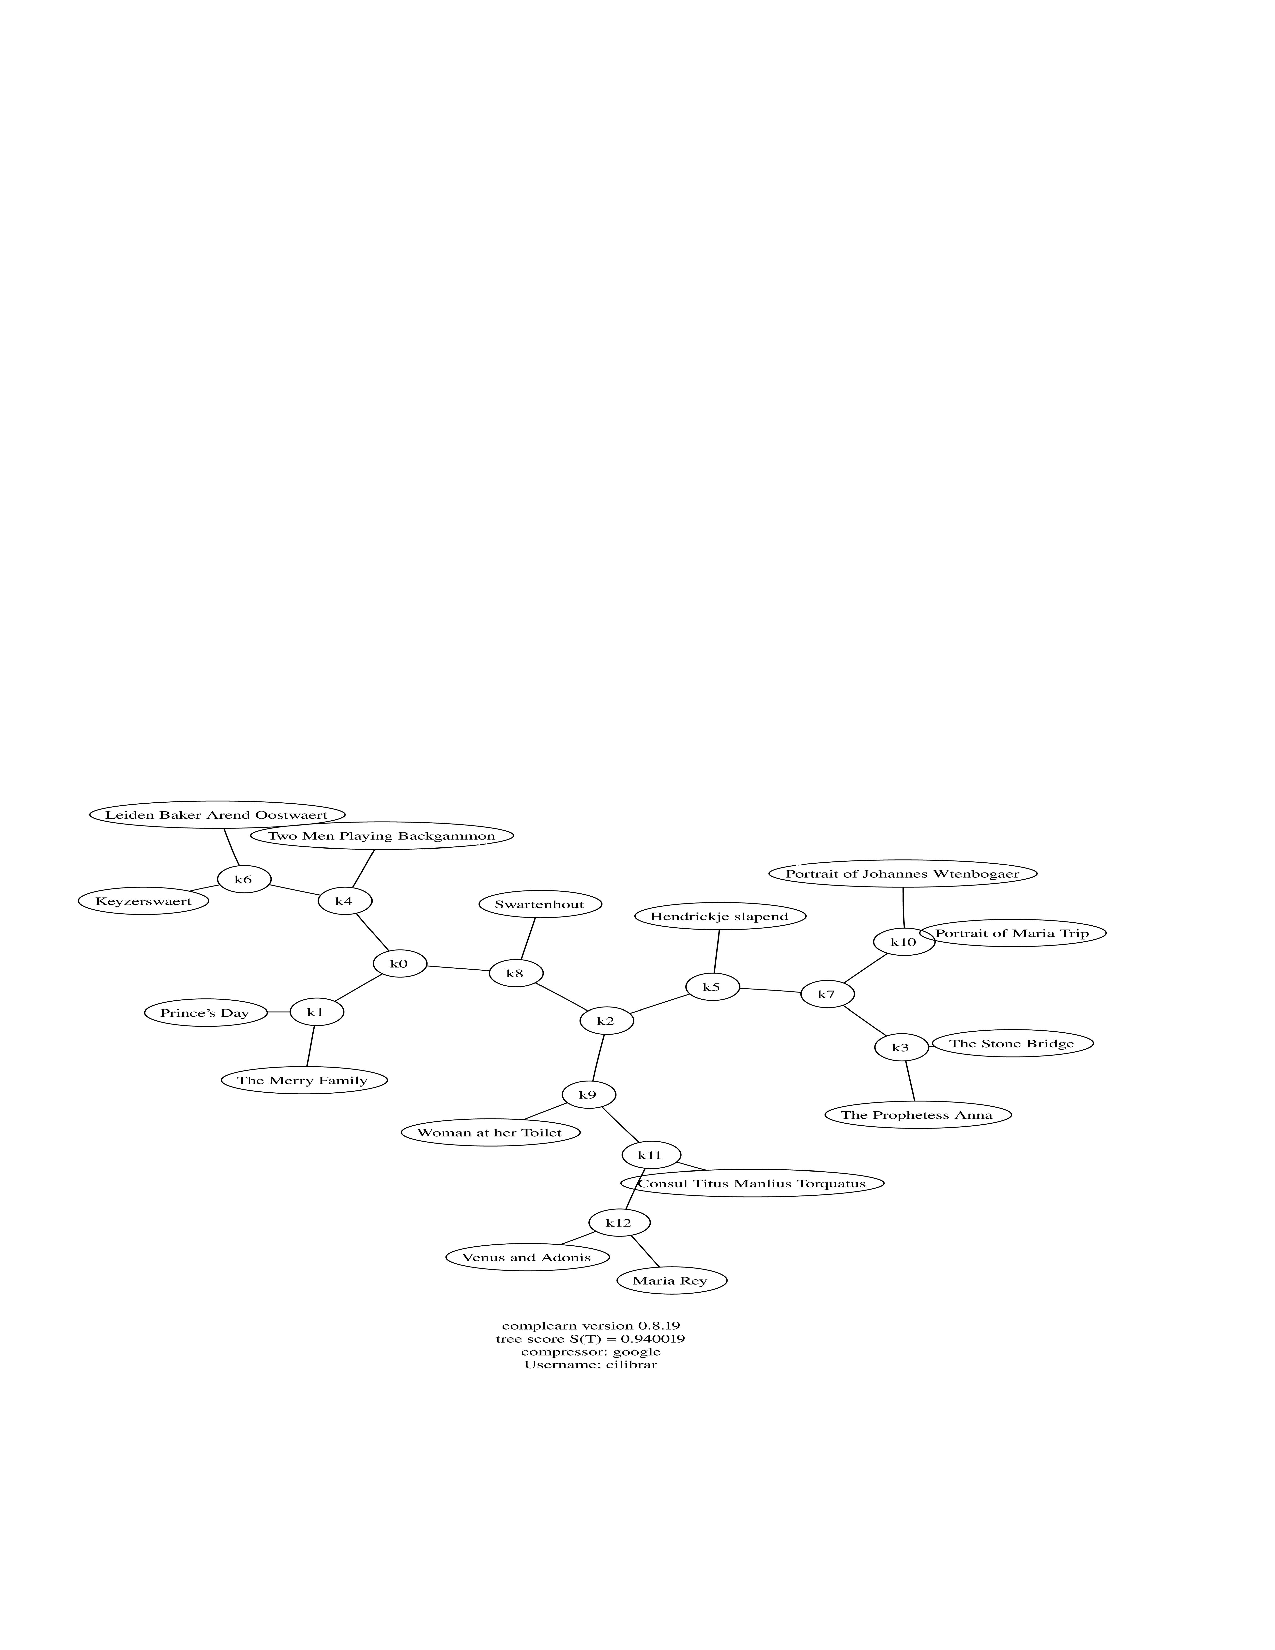
\includegraphics[width=\textwidth, height=350pt]{img/dutch-paintings}
        \caption{\emph{Hierarkkinen klusterointi hollantilaisista maalauksista} \cite{cilibrasi2007google} }
        \label{fig:dutch-paintings}
      \end{figure}

      GSD on selkeästi \cite{cilibrasi2007google} tehokas tapa klusteroida objekteja, joskin syntyvät klusterit perustuvat mielivaltaisesti internetin sisältöön, eikä objektien ominaisuuksiin.


    % subsection klusterointi (end)

  % section google_samankaltaisuusetaisyys (end)

\section{Yhteenveto} % (fold)
\label{sec:yhteenveto}

  Luvussa \ref{sec:klusterointi} näytettiin että NCD toimii hyvin klusterointiin ja on helppo soveltaa mihin tahansa alaan, kuten esimerkiksi: musiikki, kirjallisuus ja genomit, koska algoritmin käyttö on täysin riippumaton datasta ja sen ominaisuuksista. Algoritmi kykenee aina löytämään merkittävimmät ominaisuudet datasta ja vertailemaan näin samankaltaisuuden etäisyyksiä datan eri objektien välillä.
  NCD:n tehokkuutta parantaa huomattavasti että algoritmi vaikuttaa olevan hyvin kohinansietokykyinen, eli kykenee edelleen yhdistämään samankaltaisen objektit vaikka toisessa olisikin kohinaa.
  Vaikka NCD:n kehittäjät luulivat osoittaneen, että algoritmi on riippumaton pakkaajan valinnasta \cite{CV05}, niin vertailujen tuloksena on pystytty todistamaan, että ainoastaan tiedostonkokoa rajoittamaton pakkaaja toimii aidosti NCD:n kanssa \ref{sub:pakkaajan_valinta}.
  Kannattavin valinta pakkaajaksi on \emph{PPMZ}, mikäli käyttää NCD:n tuloksia klusterointiin.

  NCD ei tietenkään ole ainut menetelmä jota valvomattomassa oppimisessa voi käyttää datan klusteroimiseen.
  Hierarkkinen klusterointi on tapa jota NCD:n kanssa klusteroidessa käytetään, eli toisiaan lähemmät objektit liittyvät enemmän toisiinsa kuin kauempana olevat. Vaihtoehtoisesti voidaan käyttää K-keskiö klusterointia \engl{K-means clustering}, jossa pyritään klusteroimaan objektit $k$ eri klusteriin, klusterin keskipisteen etäisyyden perusteella; taikka jakautumaan pohjautuvaa klusterointia, jossa klusteroidaan objektit jotka todennäköisesti kuuluvat samaan jakaumaan.

  Normalisoidun pakkausetäisyyden aihealueesta on tehty paljon tutkimusta eri suuntautumishaaroihin ja tässä esitellään muutama alue, joita tämän tutkielman pohjalta voi lukea.
  Geeniekspressioanalyysi on ... ja on tutkittu NCD:n käyttöä tässä \cite{nykter2005normalized}.
  Tarkempaa tietoa normalisoidun informaatioetäisyyden ominaisuuksista ja sen epäapproksimoitavuudesta \cite{terwijn2011nonapproximability}.
  Tutkimusta on myös tehty siitä, että miten NCD toimiin kuvantunnistuksessa, asiasta lisää \cite{doi:10.1117/12.704334}.
  NCD:n kohinan sietokykyä on tutkittu ja se on avannut tutkimuksen mahdollisuuksia tälle aiheelle, tämän lisäksi on myös tutkittu miten NCD:tä voi hyödyntää kohinan poistossa \cite{vitanyi2013similarity}
  Nelikkomenetelmän tarkempaa kuvausta \cite{DBLP:journals/corr/abs-cs-0606048}


% section yhteenveto (end)
% --- References ---
%
% bibtex is used to generate the bibliography. The babplain style
% will generate numeric references (e.g. [1]) appropriate for theoretical
% computer science. If you need alphanumeric references (e.g [Tur90]), use
%
\bibliographystyle{babalpha-lf}
%
% instead.

% \bibliographystyle{babplain-lf}
\bibliography{references-fi}


% --- Appendices ---

% uncomment the following

% \newpage
% \appendix
%
% \section{Esimerkkiliite}

\end{document}
